\documentclass[a4paper,10pt,titlepage]{report}
%%This template is based on Paco van Beckhoven's thesis. 

\usepackage{tabulary}
\usepackage{xspace}
\usepackage{xargs}   % Use more than one optional parameter in a new commands
\usepackage[pdftex,dvipsnames]{xcolor}

% Putting images next to each other
\usepackage[font=bf,]{caption}
\usepackage{subcaption}
\input{glyphtounicode}

% for last page
\usepackage{lastpage}

\usepackage[english]{babel}
\usepackage[utf8]{inputenc}
\usepackage{csquotes}
\usepackage[margin=1in]{geometry}
\usepackage{fancyhdr}
\usepackage{booktabs}
\usepackage{paralist}
\usepackage{graphicx}
\usepackage{tabularx}
\usepackage{adjustbox}
\usepackage{titlepic}
\usepackage{vhistory}
\usepackage{enumitem}
\usepackage{longtable}
\usepackage[backend=biber,style=ieee,citestyle=numeric-comp]{biblatex}
\usepackage[colorinlistoftodos, prependcaption]{todonotes}
\usepackage{placeins}
\usepackage{multirow}
\usepackage{amsmath,amssymb}
\usepackage[hidelinks]{hyperref}
\usepackage[acronym,nogroupskip,nohypertypes={acronym},toc,section=chapter]{glossaries}
\usepackage{amssymb}
\usepackage{verbatim}
\usepackage{cmap}

%\usepackage[ansinew]{inputenc}
%\usepackage[T1]{fontenc}
%\usepackage{libertine}
\input{glyphtounicode}

\pdfglyphtounicode{f_f}{FB00}
\pdfglyphtounicode{f_f_i}{FB03}
\pdfglyphtounicode{f_f_l}{FB04}
\pdfglyphtounicode{f_i}{FB01}

\pdfgentounicode=1



%Appendix package + appendix in chapter title
\usepackage[titletoc]{appendix}


\usepackage{hhline}


%for highlighting findings
\usepackage{tcolorbox}

% for highlighting code examples
\usepackage{listings}

\newcommand{\ie}{\emph{i.e.},\xspace}
\newcommand{\eg}{\emph{e.g.},\xspace}
\newcommand{\etc}{\emph{etc.}\xspace}
\newcommand{\etal}{\emph{et al.}\xspace}

\newcommand{\sig}{\gls{sig}}
\newcommand{\sigs}{\glspl{sig}}

\newcommandx{\unsure}[2][1=]{\todo[linecolor=red,backgroundcolor=red!25,bordercolor=red,#1, inline]{#2}}
\newcommandx{\discussion}[2][1=]{\todo[linecolor=red,backgroundcolor=green!25,bordercolor=red,inline,#1]{#2}}

\newcommandx{\improvement}[2][1=]{\todo[linecolor=blue,backgroundcolor=blue!25,bordercolor=blue,#1]{#2}}

\newcommandx{\reminder}[2][1=]{\todo[linecolor=yellow,backgroundcolor=yellow!25,bordercolor=yellow,#1]{#2}}

\newcommandx{\lessprio}[2][1=]{\todo[linecolor=Plum,backgroundcolor=Plum!25,bordercolor=Plum,#1]{#2}}
\newcommandx{\todocontent}[2][1=]{\todo[author=\textbf{Planned content},backgroundcolor=Goldenrod!25,bordercolor=Goldenrod,inline,#1]{#2}}

\definecolor{ryel}{HTML}{fcd116}
\definecolor{rred}{HTML}{ce1126}
\definecolor{rblu}{HTML}{0a3eb9}
%these are examples of commands that may facilitate feedback annotations in the document
%replace \paco by your name and \ana by your supervisor's name
%\newcommandx{\ana}[2][1=]{\todo[linecolor=rblu,backgroundcolor=ryel,bordercolor=rred,#1]{#2}}
%\newcommandx{\paco}[2][1=]{\todo[author=Paco,linecolor=blue,backgroundcolor=white,bordercolor=red,#1]{#2}}


% -- title page is a modified version of https://github.com/software-engineering-amsterdam/latex/blob/master/thesis/uvamscse.cls
\newcommand{\email}[1]{\ttfamily\href{mailto:#1}{#1}}

\newcommand{\uvacoverfoot}{%
	\vfill
	\begin{center}
		\begin{tabular}{r|l}
			\multirow{3}{*}{
\includegraphics[height=48pt]{uva.pdf}}
			&\textsc{\Large Universiteit van Amsterdam}\\
			&\textsc{Faculteit der Natuurwetenschappen, Wiskunde en Informatica}\\
			&\textsc{Master Software Engineering}\\
			&\url{http://www.software-engineering-amsterdam.nl}
		\end{tabular}
	\end{center}
}

\renewcommand{\maketitle}{%
	% The cover page
	% --------------
	\thispagestyle{empty}
	\enlargethispage{30pt}
	\renewcommand{\thefootnote}{\fnsymbol{footnote}}
	% Will be page 0, s.t. contents start on page 1
	\setcounter{page}{0}
	% \eccoverhead
	% Volume and article title, author(s)
	\vspace{60pt}
	\begin{center}
		{\Huge\bfseries Interactive Pipeline Construction Environment for Virtual Reality Visualizations \par}
		
		\vspace{44pt}
		{\Large\bfseries Sandro Massa \par}
		\email{sandro.massa@student.uva.nl}\\
		\vspace{11pt}
		August 01, 2021, \pageref{LastPage} pages
	\end{center}
	\vfill
	\begin{tabular}{ll}
		\textbf{Academic supervisor:} 	& dr Robert G. Belleman, \email{r.g.belleman@uva.nl} \\
		\textbf{Host organisation/Research group:} & \href{http://visualisationlab.science.uva.nl/}{Visualization Lab at Science Park,} \\
		& \href{https://uva.computationalscience.nl/} {Computational Science Lab}
	\end{tabular}
	\uvacoverfoot
	\newpage
	\setcounter{footnote}{0}
	\renewcommand{\thefootnote}{\arabic{footnote}}
	\setlength{\parskip}{0pt}
}

%\newcommand{\uvaabstract}{}latex 
%\renewcommand{\abstract}[2][Abstract]{\renewcommand{\uvaabstract}{\chapter*{Abstract}%
%\par#2\newpage}}


%-------- End of ``title page''

%Fancy page headers
\pagestyle{fancy}
\fancyhf{}
\fancyhead[L]{\leftmark}
\fancyfoot[C]{\thepage}
\setlength{\headheight}{14pt}


%%FINDING ENV
\newcounter{findingctr}

\newenvironment{finding}{%      define a custom environment
	\refstepcounter{findingctr}% increment the environment's counter
	\begin{tcolorbox}
	\textbf{Finding \thefindingctr:}
}{\end{tcolorbox}} 
% If you want numbers that start with the chapter or section number (e.g. 7.1.1 or 7.1) enable the following lines 
%\usepackage{amsmath}
%\numberwithin{findingctr}{chapter}


% Decrease the size of all these lists
\setlist{noitemsep,topsep=4pt,parsep=1pt,partopsep=4pt}


\lstset{
	basicstyle=\footnotesize,        % the size of the fonts that are used for the code
	breakatwhitespace=false,         % sets if automatic breaks should only happen at whitespace
	breaklines=true,                 % sets automatic line breaking
	captionpos=b,                    % sets the caption-position to bottom
	frame=single,                    % adds a frame around the code
	language=Java,                 % the language of the code
	keywordstyle=\bf,
	tabsize=2                       % sets default tabsize to 2 spaces
}

%% Python settings from https://tex.stackexchange.com/questions/83882/how-to-highlight-python-syntax-in-latex-listings-lstinputlistings-command

% Default fixed font does not support bold face
\DeclareFixedFont{\ttb}{T1}{txtt}{bx}{n}{12} % for bold
\DeclareFixedFont{\ttm}{T1}{txtt}{m}{n}{12}  % for normal

% Custom colors
\usepackage{color}
\definecolor{deepblue}{rgb}{0,0,0.5}
\definecolor{deepred}{rgb}{0.6,0,0}
\definecolor{deepgreen}{rgb}{0,0.5,0}
\definecolor{listinggray}{gray}{0.9}
\definecolor{lbcolor}{rgb}{0.9,0.9,0.9}

% Python style for highlighting
\newcommand\pythonstyle{\lstset{
    language=Python,
    backgroundcolor=\color{lbcolor},
    keywordstyle=\color[rgb]{0,0,1},
    commentstyle=\color{deepgreen},
    stringstyle=\color{red},
    tabsize=4,
    captionpos=b,
    tabsize=3,
    frame=lines,
    numbers=left,
    numberstyle=\tiny,
    numbersep=5pt,
    breaklines=true,
    showstringspaces=false,
    basicstyle=\footnotesize,
    emphstyle=\bfseries,    % Custom highlighting style
    morekeywords={self},    % Add keywords here
    emph={os,__init__},     % Custom highlighting
}}

% Output style for highlighting
\newcommand\pythonoutputstyle{\lstset{
    language=,
    basicstyle=\ttm,
    frame=tb,
    showstringspaces=false
}}

% C++ style for highlighting
\newcommand\cppstyle{\lstset{
    language=C++,
    backgroundcolor=\color{lbcolor},
    keywordstyle=\color[rgb]{0,0,1},
    commentstyle=\color{deepgreen},
    stringstyle=\color{red},
    tabsize=4,
    captionpos=b,
    tabsize=3,
    frame=lines,
    numbers=left,
    numberstyle=\tiny,
    numbersep=5pt,
    breaklines=true,
    showstringspaces=false,
    basicstyle=\footnotesize,
    emphstyle=\bfseries,    % Custom highlighting style
    emph={LPCSTR, std, stringstream, T, vtkSmartPointer, vtkActor, VtkAdapter, VtkAdapterUtility, unordered_map, VtkConeSource, VtkConeSourceAdapter, Singleton, vtkQuadric, vtkSampleFunction, vtkNew, vtkContourFilter, vtkPolyDataMapper, vtkOutlineFilter, vtkRenderer, vtkRenderWindow, vtkRenderWindowInteractor, EXIT_SUCCESS},
}}


% Python environment
\lstnewenvironment{python}[1][]{
    \pythonstyle
    \lstset{#1}
}{}

% Output environment
\lstnewenvironment{pythonoutput}[1][]{
    \pythonoutputstyle
    \lstset{#1}
}{}

% Cpp environment
\lstnewenvironment{cpp}[1][]{
    \cppstyle
    \lstset{#1}
}{}

% Python for external files
\newcommand\pythonexternal[2][]{{
    \pythonstyle
    \lstinputlisting[#1]{#2}
}}

% Output for external files
\newcommand\pythonoutputexternal[2][]{{
    \pythonoutputstyle
    \lstinputlisting[#1][#2]
}}

% Cpp for external files
\newcommand\cppexternal[2][]{{
    \cppstyle
    \lstinputlisting[#1][#2]
}}

% Python for inline
\newcommand\pythoninline[1]{{\pythonstyle\lstinline!#1!}}

% Output for inline
\newcommand\pythonoutputinline[1]{{\pythonoutputstyle\lstinline!#1!}}

% Cpp for inline
\newcommand\cppinline[1]{{\cppstyle\lstinline!#1!}}

%make it fit more nicely
\setlength\extrarowheight{2pt}

%for subfiguring
\usepackage{caption}
\usepackage{subcaption}


%helpful acronym examples
%% \newacronym{cc}{CC}{Cyclomatic Complexity}

%% \newacronym{sut}{SUT}{System Under Test}

%% \newacronym{strew}{STREW}{Software Testing and Reliability Early Warning}

%% \newacronym{sig}{SIG}{Software Improvement Group}

%% \newacronym{sat}{SAT}{Software Analysis Toolkit}

%% \newacronym{tloc}{TLOC}{Lines Of Test Code}
%% \newacronym{loc}{LOC}{Lines of Code}

%% \newacronym{taime}{TAIME}{Test Suite Assessment and Improvement Method}

%% \newacronym{tqm}{TQM}{Test Quality Model}

%% \newacronym{tdd}{TDD}{Test-Driven Development}

%% \newacronym{cor}{COR}{Conditional Operator Replacement}
%% \newacronym{ror}{ROR}{Relational Operator Replacement}
%% \newacronym{ast}{AST}{Abstract Syntax Tree}

\newacronym{vr}{VR}{Virtual Reality}
\newacronym{vtk}{VTK}{The Visualization ToolKit}
\newacronym{itk}{ITK}{The Insight ToolKit}
\newacronym{fps}{FPS}{frames per second}
\newacronym{ide}{IDE}{Integrated Development Environment}
\newacronym{gpge}{GPGE}{General Purpose Game Engine}
\newacronym{hmd}{HMD}{Head-Mounted Display}
\newacronym{uva}{UvA}{University of Amsterdam}
\newacronym{ui}{UI}{User Interface}
\newacronym{ux}{UX}{User Experience}
\newacronym{slocs}{SLOCs}{Source Lines of Code}
\makeglossaries
\bibliography{main}

\begin{document}



\maketitle
\chapter*{Abstract}

Developing VR visualizations is an iterative process that requires the developer to move between workstation and testing area. The usage of Head Mounted Displays that require the user to fully move away from development and immerse themselves into the environment can make the experience tiring and break flow of development. Furthermore, no tools exist to streamline the development of such visualizations, requiring the user to have a set of technical skills that make approaching this world harder.

We present a new architecture for integrating visualization libraries such as VTK with game and simulation engines like Unity, that allows users to have an out-of-the-box integration and development environment, reducing the technical barrier for such development. The architecture tackles both the low level integration of the two softwares, as well as the creation of a UI framework to allow the user to build and interact with visualizations.

Finally, we present the implementation of such an integration that is able to leverage the full potential of the visualization library while achieving the required performances for a VR app, showing that the proposed architecture is capable of supporting an immersive VR environment for the development of VR visualizations which would remove the obstacles and issues of traditional desktop development.

\tableofcontents
\chapter{Introduction}
\label{ch:introduction}
%% Context: what is the bigger scope of the problem you are trying to solve? Try to connect to societal/economical challenges.
%% Problem Analysis: Here you present your analysis of the problem situation that your research will address.
%% How does this problem manifest itself at your host organisation?
%% Also summarises existing scientific insight into the problem.


\acrfull{vr} offers great opportunities, especially when it comes to visualizing information and applications, that enable students, practitioners and researchers to better understand and manipulate data. The main advantages over classic screens are its capacity of creating fully interactive and immersive environments, as well as leveraging the human innate spatial comprehension and interaction capabilities \cite{belleman_interactive_2003}. These make \acrshort{vr} suited for all applications where interaction and immersion are critical, ranging from educational \cite{hussein_benefits_2015} to medical \cite{faria_benefits_2016, chen_psychological_2009} purposes. Another important aspect of \acrshort{vr} that arises directly from its interactive and immersive environments, is that it has good support for activities that require the user to stay active, such as didactic and educational activities. \cite{hussein_benefits_2015}.

%TODO: vedi  itk
To aid creating visualizations, both for \acrshort{vr} and not, a number of toolkits and frameworks exist. Focusing on scientific visualization, there are several toolkits such as \acrfull{vtk} and \acrfull{itk}. \acrshort{vtk} is a powerful and extensive open source toolkit for (3D) visualization, is a widely known and used library which is based on the creation of visualization pipelines \cite{schroeder_visualization_2006}. \acrshort{itk} \cite{mccormick_itk_2014} instead, offers libraries in a variety of programming languages focused on creating visualization for different purposes. Examples are volume rendering \cite{wheeler_virtual_2018, drebin_volume_1988} for medical and engineering purposes and parallel model computation and rendering \cite{dutra_distributed_2007}. As such, these toolkits become also an important resource for \acrshort{vr} environments' development \cite{wheeler_virtual_2018}.

A number of tools already exist for development with these libraries: environments such as ParaView\footnote{\url{https://www.paraview.org/}}, MeVisLab\footnote{\url{https://www.mevislab.de/}} and DeVIDE \cite{botha_devide_2004} integrate either one or the other or both and more of these toolkits. Even though some integration exists for \acrshort{vr} development \cite{sua_virtual_2015, shetty_immersive_2011}, these fall short of making use of the powerful capabilities of \acrshort{vr} and are only portings. These still require the user to jump in and out of the environment to make adjustments at the desktop workstation and can be both wasteful in time and break workflow \cite{belleman_interactive_2003, dreuning_visual_2016, kruis_creating_2017, schutte_virtual_2018}. Coupled with the fact that development of good visualizations is an iterative process, requiring the developer to tweak the pipeline multiple times over, it makes for an inefficient process at best.

This thesis proposes a way of integrating these toolkits, in particular focusing on \acrshort{vtk}, with general purpose \acrshort{vr} applications development environments, both lowering the technical barrier of using these toolkits and their restrictions when it comes to \acrshort{vr}, as well as making use of the capabilities this technology has to offer. To achieve this, we look at previous attempts with this toolkit and its existing environments \cite{dreuning_visual_2016, kruis_creating_2017, schutte_virtual_2018}, other environments \cite{wheeler_virtual_2018} and similar specific \acrshort{vr} development environments \cite{vanhorn_deep_2019}.

We develop a \acrshort{vr} pipeline development environment inspired by ParaView desktop's approach, where the user is able to both edit and render the visualization without exiting the VR environment and using an intuitive block-based editor to create the pipeline. More specifically, we develop an integration between the \acrshort{vtk} library and Unity, a general purpose game engine \cite{haas2014history}, that is used for the generation of the virtual world, as well as handling the UI components that allow editing of the \acrshort{vtk} objects.

\section{Problem statement}

Creation of \acrshort{vr} visualizations in particular is, to this day, cumbersome, requiring the user to mostly work from a desktop screen, which is not ideal to design a \acrshort{vr} visualization, due to its different nature. Another big issue is the fact that to move between testing and usage station (i.e. the \acrshort{vr} headset, and the desktop development station) is a non-trivial job that is time consuming at best, and at worst a factor slowing down and degrading the development process. Creating such an environment represents an important step for the visualization community, removing barriers for \acrshort{vr} development, and a challenge from a Software Engineering stand point. Furthermore, from a research perspective a number of questions open up which are not yet fully explored.

A key characteristic of any good \acrshort{vr} environment is performance: in order to have a decent user experience, and limit the influences of motion sickness and other problems that arise from poorly designed \acrshort{vr} environments \cite{viire1997health}, the software needs to reach high performance thresholds. Guidelines for general applications for \acrshort{vr} suggest to achieve a framerate of at least 90 FPS \cite{unity_vr_2020}, but depending on the headset even higher framerates may be needed, i.e. with newer versions of the Valve Index or the Pimax 5K plus. Considering that a \acrshort{vr} \acrfull{hmd} is made of two displays, one per eye, the target FPS is double the suggested threshold, posing serious design challenges.

\subsection{Research questions}

Designing an environment as the one we describe opens up a number of questions, especially what are the challenges with it its maintainability, as it involves connecting two third-party code bases. We investigate similar works in order to fully develop a stable core of the environment we envision. A very first step has already been accomplished by finding ways to embed visualization libraries in visualization engines that is the base of our environment. Examples of this are ActiViz \cite{kitware_activiz} and Wheeler et al.'s VtkToUnity \cite{wheeler_virtual_2018}, both interfacing \acrshort{vtk} with Unity.

These solutions though aim not at creating development environments, but are oriented at supporting the development of specific applications. For example ActiViz is a commercial tool which has performance limits due to its use of copying operations from CPU to GPU \cite{gregg2011data}, whereas Wheeler et al.'s VtkToUnity, part of the 3DHeart project \cite{wheeler_virtual_2018}, lacks generality, as \acrshort{vtk} is called through specialized code and only the \acrshort{vtk} feature needed are actually visible from Unity.

\begin{itemize}[leftmargin=1.5truecm]
    \item[\textbf{RQ1}] In what way can interfacing \acrlong{vtk} with Unity Game Engine be done such that \acrshort{vr} usability and performance standards are upheld?
\end{itemize}

By fully interfacing the toolkit with the game engine we intend that the engine has full access to the capabilities of \acrshort{vtk}, while this last one is able to capture events arising within the environment. From previous attempts at achieving this \cite{dreuning_visual_2016, kruis_creating_2017, schutte_virtual_2018, wheeler_virtual_2018}, we found that a major issue comes from using different versions of the involved libraries, which were not always traceable back to a simple API change. As such, our intent is to investigate what factors contribute to this instability and how we can limit their impact on the solution.

\begin{itemize}[leftmargin=1.5truecm]
    \item[\textbf{RQ2}] What are the factors contributing to maintainability issues of interfacing \acrlong{vtk} and Unity Game Engine?
    \begin{itemize}[leftmargin=1.5truecm]
        \item[\textbf{RQ2.1}] How can the impact of these factors on the maintainability of the system be limited?
    \end{itemize}
\end{itemize}

Finally, as \acrshort{ui} and \acrshort{ux} are out of the scope of this thesis, yet important to our successful investigation of the aforementioned research questions, thus they are investigated alongside this thesis project by someone else. Due to the constraints on a work such as a Master's Thesis, we report on the difficulties of such a Software development Process.

\subsection{Research method}

In order to investigate our research questions, we design a software system based on precedent work. The design is guided by three main principles which reflect the constraints we put in our research questions:

\begin{enumerate}
    \item \textbf{Integration}: the two main components of the system we develop already exist, \acrshort{vtk} and Unity. A link between the two exists, but is imperfect, and does not allow the capabilities of both to be fully leveraged in the end system. This may be sufficient for some applications, but where a full interfacing of the two is necessary, the existing approaches require a great development overhead. Our objective is to reduce this overhead by maximizing the integration between these two components;
    
    \item \textbf{Performance}: a key problem with \acrshort{vr} applications is achieving the performances that are sufficient for a decent user experience. A number of guidelines exist on what these performances should be in terms of \acrfull{fps} 
    %FIXME: hai parlato di fps prima, qui basta l'acronimo breve
    \cite{unity_vr_2020,epic_virtual_2021}. As we set out to create a usable \acrshort{ide} that should be usable by users to create their visualizations within a \acrshort{vr} environment, we have the objective of achieving an average \acrshort{fps} count of the recommended values for the game engine we select. Another critical aspect of performance is response time: queries and operations on the pipeline have to be executed as fast as possible to avoid rendering issues and long waiting periods.
    
    \item \textbf{Maintainability}: as previously expressed, one of our main concerns is maintainability. Due to the nature of the system we develop, our concern is to maximize its maintainability for long term support. We first and foremost investigate which factors contribute to hardly maintainable solutions and we then discuss how we can limit them.
\end{enumerate}

Given these drivers, and our goal of creating a long-lasting \acrshort{ide} that would enhance the quality of life of the \acrshort{vr} visualization development community. Our first concern is to investigate the factors contributing to the maintainability issues of previous solutions proposed by performing a small literature review, collecting a number of previous solutions, and examining them to find out their weak spots. We compile a list of these factors and how much they impact the system, how easily they can be avoided or solved and what components they involve.

Based on the results of this first part, we design an architecture with the objective of minimizing the factors impacting maintainability. At this stage, we also focus on laying the grounds of a performing system, and as such we discuss a number of design choices, potentially based on architectures from different strands of Computer Sciences. We attempt to keep the concerns as separate and encapsulated as possible with the intent of enabling the software to be distributed.

Finally, we develop a proof of concept that we test for performance on a number of visualizations on three main operations: creation of the visualization, rendering of the visualization and a combination of the two. We then compare the results of our benchmarks with the guidelines provided by the developer of Unity and/or manufacturer of the \acrshort{vr} headset we choose, as well as with the results of previous research on this topic \cite{dreuning_visual_2016, wheeler_virtual_2018}.

Alongside this main research journey, we also collect, in the form of Action-Research, a diary of the difficulties we encountered in researching, designing and implementing the software, as well as managing the two different development branches that are to be highly decoupled. Based on our experience, we discuss what were the weak points of our approach and what are in hindsight potential precautions and solutions we could have taken to enhance productivity and success chances.

\section{Contributions}

Our research makes the following contributions:

\begin{enumerate}
	\item Analysis of the factors contributing to the unmaintainability of software bridging \acrshort{vtk} and Unity,
	\item Development of a potentially distributed architecture for performing \acrshort{vr} visualization creation and rendering systems,
	\item Insight into the preparation, development and management of software where developers work on depending components with the constraint of having decoupled work.
\end{enumerate}

\section{Outline}

In Chapter~\ref{ch:background} we describe the background of this thesis and analyse previous work researching factors contributing to maintainability issues of this kind of software. Chapter~\ref{ch:rqrmsandclngs} describes the design challenges and choices of the system. Chapter~\ref{ch:design} describes the development of an architecture able to support the performance required by our software while meeting its requirements. Benchmarks are briefly introduced in Chapter~\ref{ch:materials}. Results of the literature review, development, testing and benchmarking are shown in Chapter~\ref{ch:results} and discussed in Chapter~\ref{ch:discussion}. Finally, we present our concluding remarks in Chapter~\ref{ch:conclusion} together with future work.


\chapter{Background}
\label{ch:background}

This chapter presents the necessary background information for this thesis. First, we define some basic terminology that we use throughout this document. Next, we research prior work in the field of \acrshort{vr} that interfaces \acrshort{vtk} and Unity or develops \acrshort{ide}s for visualizations within a \acrshort{vr} environment. We also examine the software and solutions produced by these previous studies and extract which factors contribute to potential maintainability issues and which on the contrary make them more maintainable. 

\section{Terminology}

We define a set of terms that we use throughout this thesis. We use the \textit{Glossary of virtual reality terminology} \cite{manetta1995glossary} as a main source for our terminology.

\begin{itemize}[leftmargin=1.5truecm]
    \setlength{\itemindent}{-1truecm}
    \item[] \textbf{\acrfull{vr}} A computer system used to create an artificial world which is immersive and interactive for the user.
    \item[] \textbf{Immersion} The feeling of the user of being part of a virtual environment.
    \item[] \textbf{Virtual Environment} Realistic simulations of interactive scenes.
    \item[] \textbf{Interactivity} The ability of the user to navigate and manipulate (objects in) the environment.
    \item[] \textbf{Visualization Toolkit} Library containing functionality aimed at creating and manipulating data visualizations.
    \item[] \textbf{Game Engine} A software that enables the creation of virtual environments.
\end{itemize}

\section{The Visualization Toolkit}

As the necessity to produce ever more complex visualizations grows, both in commercial and scientific settings, a number of visualization toolkits have been developed to support the development of these visualizations. These libraries tend to specialize on some form of visualization; for example, \acrfull{vtk} focuses on scientific visualization \cite{kruis_creating_2017}.

These toolkits come in a variety of flavours, languages and/or wrappings and it is thus out of the scope of this thesis to analyse and develop upon all of them. We discuss research done on all three to create \acrshort{ide}s for or within \acrshort{vr} environments, but we ultimately choose to use for a proof of concept.

\acrfull{vtk} is a library oriented towards \blockquote{\textit{manipulating and displaying scientific data}}\footnote{\url{https://vtk.org/}}. It creates visualizations by means of filter pipelines, a technique proposed by Haber and McNabb \cite{haber1990visualization}. These filters manipulate input data through some set of transformations and return the composed data which can then be visualized. 

\acrshort{vtk} has three different stages of the pipeline which combined return a visualization rendering. The first stage is the generation or the import of a data source and transforming the raw data in some more readable raw data if needed, like structuring it in a model. Subsequently, the raw data is then transformed through filters that compose the data in order for it to be visualized, creating the actual visualization. Finally, the visualization is rendered through the application of mappers that transform the computational representation into a graphical representation. An example of a Quadric 3D function is shown in Figure~\ref{fig:quadric-render-pipeline}, based on an example proposed in the \acrshort{vtk} example repository\footnote{Available at \url{https://kitware.github.io/vtk-examples/site/Cxx/VisualizationAlgorithms/ContourQuadric/}.}, the exact code is presented in Appendix~\ref{apx:quadric-vtk}.

\begin{figure}[t]
    \centering
    \begin{subfigure}{\textwidth}
        \centering
        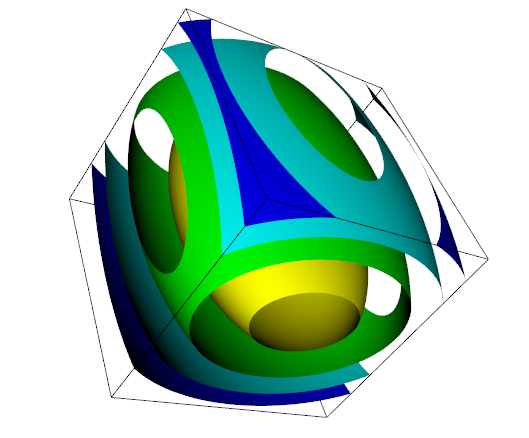
\includegraphics[width=0.7\textwidth]{pictures/Quadric-Rendering.PNG}
        \caption{}
    \end{subfigure}
    \begin{subfigure}{\textwidth}
        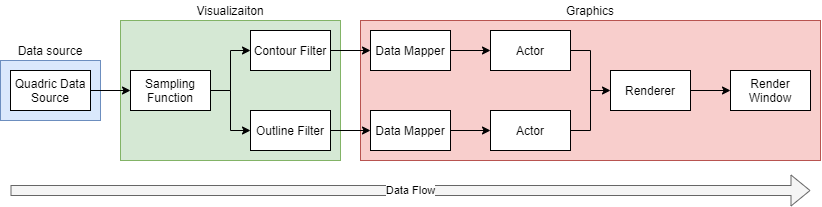
\includegraphics[width=\textwidth]{pictures/Pipeline-VTK-Quadric.png}
        \caption{}
    \end{subfigure}
    \caption{VTK visualization (a) and pipeline (b) of a sampled Quadric function.}
    \label{fig:quadric-render-pipeline}
\end{figure}

Upon \acrshort{vtk}, a number of wrappers have been produced, allowing the library to be used not only in C++, but also in Java, Python, Tcl and the .NET Framework\footnote{\url{https://vtk.org/Wiki/VTK/Wrappers}}. These wrappers allow the usage of the \textit{wrappable} code of the library from one of the aforementioned languages. This process is to be manually done at build time of the library or using one of the wrapping tools accessible from the documentation of \acrshort{vtk}.

\section{Unity Game Engine}

Game Engines can be defined as "\textit{software frameworks for game development}" \cite{politowski2021game}. These frameworks though are not all equal, and as such we focus on those defined as \textit{\acrfull{gpge}s}, which we define as \textit{frameworks for the creation of virtual environments}, which is a fundamental component of games. This also means that these softwares are not restricted to game development purposes, but are used for a variety of projects that entail the simulation of virtual worlds. These frameworks perfectly fit our requirement of creating an immersive and interactive environment for our \acrshort{vr} IDE.

A number of \acrshort{gpge}s exist, such as Unity Engine \cite{haas2014history} and Unreal Engine \cite{unrealengine}. We use Unity as the engine on which we base our solution. This is ideal for our research as previous research already exists discussing the integration of \acrshort{vtk} and this engine \cite{wheeler_virtual_2018}. Furthermore, it is a very well established, used and supported engine.

We chose to use Unity due to the number of advantages that come with the engine. First and foremost, Unity has already a decent \acrshort{vr} integration with the OpenVR\footnote{\url{https://github.com/ValveSoftware/unity-xr-plugin}} and OpenXR\footnote{\url{https://docs.unity3d.com/Packages/com.unity.xr.openxr@0.1/manual/index.html}} plugins. The \acrshort{vr} community is already quite established and, in general, the development community is very active and offers valuable support. 

The documentation for the engine is comprehensive and freely available with a number of examples that facilitate development, and its API supports the implementation of custom native C++ code through easy drag-n-drop of the shared libraries in the editor and an intuitive interface to import its functionalities in C\#. Finally, thanks to OpenGL 2 context sharing, it is possible to render through external code, such as \acrshort{vtk}, which suites our need to visualize objects created in native C++ libraries.

\section{HTC Vive Headmounted Display}

Our objective is to have a generic environment that can be used with any HMD. For our development, however, we focus on the HTC Vive series as these are the HMDs we have access for development and testing. These VR headsets have a 90 Hz refresh rate on the entire line and can be used with controllers, allowing for interactive usage. In particular we focus on the HTC Vive, that we use for both development and testing. This headset is shown in Figure~\ref{fig:htc-vive}

\begin{figure}[t]
    \centering
    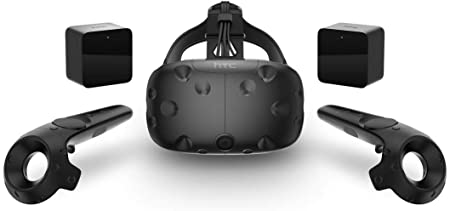
\includegraphics[width=.7\textwidth]{pictures/htc_vive.jpg}
    \caption{HTC Vive HMD with cameras and controllers.}
    \label{fig:htc-vive}
\end{figure}

\section{Related Work}
\label{sec:related-work}

A number of projects already attempted interfacing visualization libraries with frameworks, be it \acrshort{gpge}s or IDEs, while others attempted the creation of visualization editors, albeit for different purposes and/or constraints. In this section we discuss these previous attempts and how they contribute to laying the ground for our development.

\paragraph{OculusVTK Visual editor}

, developed in 2016, is a similar attempt to create a visual editor for OculusVTK carried out in Python \cite{dreuning_visual_2016}. The solution allows the user to create simple pipelines and manipulate them within a visual environment and see the result of the operations. The authors carry out a number of experiments with pipelines, varying from simple arrows to stream tracers and a DICOM image rendering, where results showed a consistent 58-60 FPS were achieved.

While the objectives of the authors are quite similar to ours, they do not focus on the same constraints we set for our project, i.e. performance and the designing of a distributable and parallelizable architecture. Furthermore, their solution focuses on Oculus, whereas our solution aims at being headset-agnostic.

The power of the solution proposed lays in its usage of Python's capability of introspecting on its modules and harvesting data in order to achieve a more general approach to interfacing with \acrshort{vtk}. We base our solution partly on this software, as we discuss in Section~\ref{sec:design-introspection}.

% Cannot find any reference of OculusVTK outside of one SURFsara webpage and Dreuning's and Perlee's theses.
On the other hand, this solution is limited to the usage of the OculusVTK C++ boilerplate for OculusVR. The code is maintained by SURFsara and offers an extension of the OculusVR SDK for Oculus HMDs. Compared to the support of Unity, this limits the generality of the solution, which we aim at extending.

Also due to the usage of OculusVTK, the solution proposes a complex building system prone to errors and issues related to building platforms, versions and library installations. Our objective is to streamline the building of our solution, if any is needed, and make our solution version-agnostic towards its dependencies. 

Furthermore, the Python scripts are limited to only working through introspection on \verb|vtkAlgorithm| subclasses, which limits the user to using such powerful tool on a subset of all available features of VTK. We aim at a general solution, thus either extending the approach up to any \verb|vtkObjectBase| subclass or to allow access to other features through the offered API.

\paragraph{VtkToUnity} is the closest attempt to our project was presented in 2018 by Wheeler et al. \\
\cite{wheeler_virtual_2018}. who developed a Native Unity plugin that allowed the user to exploit \acrshort{vtk}'s features in the engine's scripts\footnote{\url{https://gitlab.com/3dheart_public/vtktounity}}. The plugin's aim is to introduce volume rendering through \acrshort{vtk} and uses the OpenGL context sharing technology to enable the visualization library to directly render within the Unity scene. The plugin's approach is to add a rendering callback function after the transparency rendering stage, as optimal for volume rendering. The produced architecture is summarized in Figure~\ref{fig:wheeler-architecture} 

\begin{figure}[t]
    \centering
    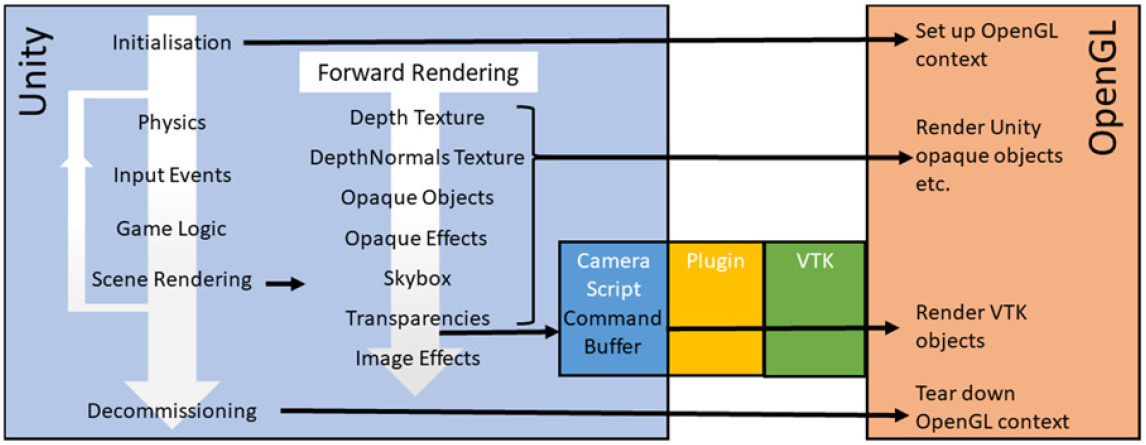
\includegraphics[width=\textwidth]{pictures/wheeler_arch.PNG}
    \caption{Wheeler et al.'s rendering architecture.}
    \label{fig:wheeler-architecture}
\end{figure}

The authors carry out experiments to evaluate the performances of the solution. Their objective frame rate is of 90 FPS using a HTC Vive \acrfull{hmd}, which aligns with Unity's own guidelines \cite{unity_vr_2020} as well as the 90Hz refresh rate of the \acrshort{hmd} \cite{BuyVIVEH54}. With simpler renderings the solution is of its own able to achieve the desired frame rate, but with more complex scenes it does not. To overcome this, the authors propose the usage of setting the desired frame rate using \acrshort{vtk}'s own \verb|vtkExternalRenderingOpenGLRenderWindow::SetDesiredUpdateRate| to solve this.

This solution presents some limitations, as the C++ native code locks the shared API at every call, and as such limits the ability to leverage parallelization of the software, which could potentially aid the rendering quality while the objective frame rate is set. Furthermore, the plugin focuses on volume rendering in particular, while our solution aims at a more general solution.

An issue with the maintainability of the VtkToUnity plugin is its hardcoding of features and reliance on patches to \acrshort{vtk}'s code to make it work correctly. For a specific application this is not a problem, but as our objective is to offer a generic solution to access VTK from Unity, this is not viable, as it introduces couplings to versions and particular algorithms and pipelines, and the potential for bugs and clones.

Our solution aims at creating a bridge that would allow the user to create pipelines in Unity without having hardcoded features limiting the user capabilities.

\paragraph{ActiViz}\footnote{\url{https://www.kitware.eu/activiz/}} is a \acrshort{vtk} wrapper for .NET, developed by Kitware, the company that is also mantaining \acrshort{vtk}. This wrapper is ready to be used with Unity, and exposes the same functionality of the library as other wrappers. This allows already for a good integration of the library and Unity.

The downside of this solution is its performance: as the wrapper requires CPU to GPU copies, with complex visualizations the performances drop significantly. This has already been discussed by Wheeler et al. \cite{wheeler_virtual_2018} and is one of the reasons that lead them to develop their own solution. On the other side, this is an official wrapper maintained by Kitware, the same creators of \acrshort{vtk}, and it has already an integration for Unity.

\paragraph{ParaView} \footnote{\url{https://www.paraview.org/}} is an \acrshort{ide} for the creation of visualizations mainly based on \acrshort{vtk}, also developed by Kitware. This uses the same paradigm as \acrshort{vtk} for the creation of visualizations, that is by the means of pipelines. An example of a ParaView visualization can be seen in Figure~\ref{fig:paraview} The software supports a \acrshort{vr} porting for the visualizations which feels clunky, as it is a rendering of 2D UIs in a 3D immersive and interactive environment, which hinders user experience.

\begin{figure}
    \centering
    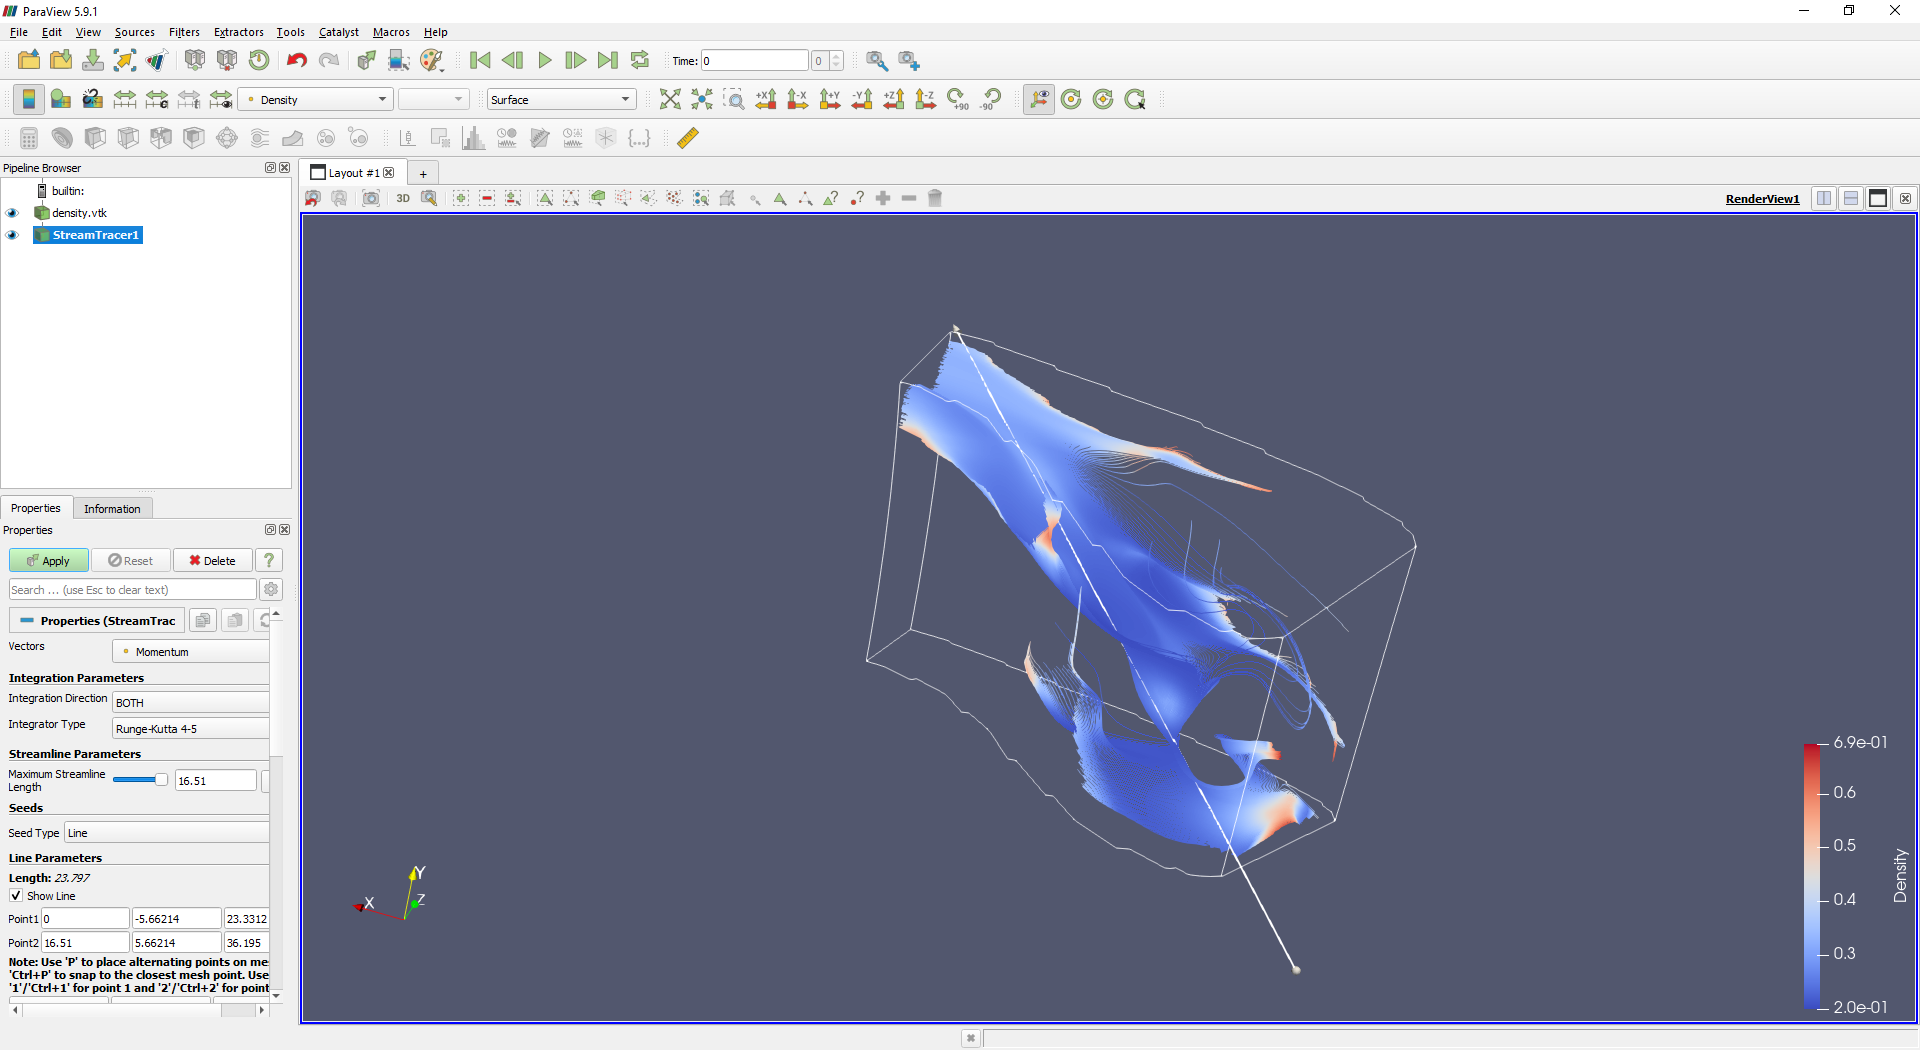
\includegraphics[width=\textwidth]{pictures/paraview.png}
    \caption{ParaView visualization of a StreamTracer using a structured grid point dataset.}
    \label{fig:paraview}
\end{figure}

Of the previous solutions, only Dreuning's work addresses the issue of allowing the creation of an integrated development environment in \acrshort{vr}. This is not an issue in and of itself, but it makes for a cumbersome and time consuming development environment for \acrshort{vr} applications. The solutions all miss one of the key characteristics we envision for our environment, be it the performances necessary for \acrshort{vr} applications, the generality of an \acrshort{ide} or the support for multiple \acrshort{hmd}s.

\chapter{Complexity Factors}
\label{ch:unmaintainability}

After analysing the different approaches taken by previous work, we define a number of requirements and challenges our solution has to meet and overcome. Most of these generate complexity in the system, and make for potential issues for long term support of such a system. As such, starting with the analysis of these issues, we focus our attention on the maintainability issues related with this project.

\section{Generality}
\label{sec:complexity-generality}

To lower the coupling between our software and \acrshort{vtk}, we want it to be version-agnostic. This coupling is already weakened by the fact the library is developed to be backwards-compatible and the only major change to the API that broke this, happened between versions 4 and 6 of the library\footnote{\url{https://vtk.org/Wiki/VTK/VTK\_6\_Migration/Overview}.}. 

We also aim at enabling the user to exploit the library to its full potential, limiting the components that cannot be reached from within the development environment, and that require technical knowledge to be integrated through code. As we discussed in Section~\ref{sec:related-work}, both the OculusVTK implementation by Dreuning and the ActiViz plugin have this capability. The first is, however, limited to Python and using OculusVR supported \acrshort{hmd}s, whereas the second is limited by its performances. 

Hardcoding \acrshort{vtk}s features would make for the best performances, but would make the system plugin a huge collection of functions, as it would be necessary to wrap the calls for every class and method accessible to the user. This approach would potentially be the more performant, but hardly makes for a maintainable system.

Instead, our approach aims to integrate Dreuning's Python introspection scripts within a C++ native plugin, as this would still allow for a performing system written in C++ to access Python's capabilities when it is necessary to expose parts of \acrshort{vtk} the system has no direct access to.

Introducing these Python scripts within the C++ plugin can be achieved through two different approaches: keeping the Python component separate and make it communicate with the C++ native plugin or embedding the Python interpreter within the C++ code itself. 

Although the first option would make for better separation of concerns, it introduces a non-trivial issue with memory sharing, synchronization, and performance. As the two parts would need to communicate, both should be able to read and write the \acrshort{vtk} objects being handled while keeping execution time as low as possible. Although, these operations can achieve the required performances of completing a full cycle in around 11.1 ms (90 \acrshort{fps} for most \acrshort{hmd}s is the recommended refresh rate), comprising of updating both lenses' views, they require careful crafting and optimizing, introducing design and code complexities.

On the other hand, the embedding of the Python interpreter is a common choice and is discussed in the official guidelines of Python itself\footnote{\url{https://docs.python.org/3/extending/embedding.html}} and can achieve decent performances. In order to determine the overhead introduced by the embedding, we compare the execution times of an embedded application with the same application in pure Python and repeat this for direct access to \acrshort{vtk} and using the Dreuning's introspection scripts.s

The application we run is a stream tracer of a density dataset for \acrshort{vtk} applications. The final visualization is composed of the outline and the streamlines. The pipeline can be seen in Figure~\ref{fig:streamtracer_pipeline}. This pipeline has been implemented in Python 3.7 directly using the \acrshort{vtk} library and accessing it through a modified and expanded version of Dreuning's scripts, the embedded verion of the Python interpreter in C++ executing Python calls directly to \acrshort{vtk}, and finally again through C++ by calling the functionality exposed by the modified Dreuning's scripts. The code for each of these tests is presented in Appendix~\ref{apx:streamtracer-performance-tests} and the results are shown in Table~\ref{tab:streamtracer-performance-tests-results}.

\begin{figure}[ht!]
    \centering
    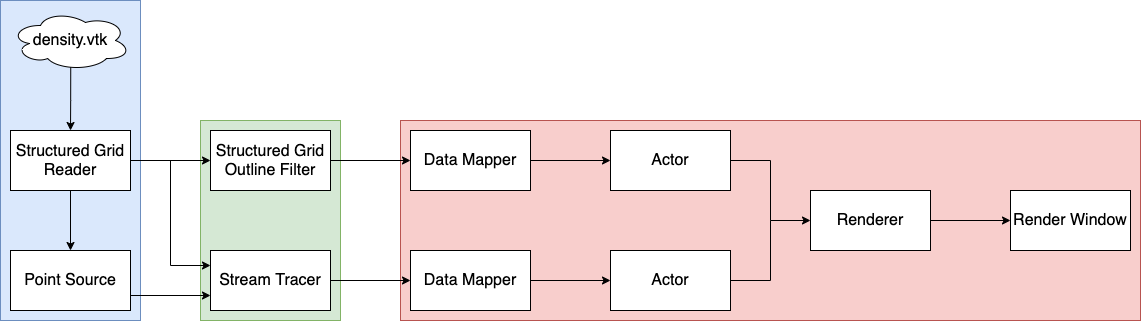
\includegraphics[width=\textwidth]{pictures/streamtracer_pipeline.png}
    \caption{VTK pipeline of a Stream Tracer on a density dataset.}
    \label{fig:streamtracer_pipeline}
\end{figure}


\begin{table}[ht!]
    \centering
    \begin{tabular}{lllll}
    \hline
    \multicolumn{1}{c}{\multirow{2}{*}{\textbf{Operations}}} &
      \multicolumn{2}{c}{\textbf{Python}} &
      \multicolumn{2}{c}{\textbf{C++}} \\ 
    \multicolumn{1}{c}{} &
      \multicolumn{1}{c}{\textbf{Native}} &
      \multicolumn{1}{c}{\textbf{Introspection}} &
      \multicolumn{1}{c}{\textbf{Native}} &
      \multicolumn{1}{c}{\textbf{Introspection}} \\ \hhline{=====}
    Loading*                       & \multicolumn{1}{l}{0}         & 1.8973614 & 0.7491320 & 2.7688682 \\
    Object instantiation**         & \multicolumn{1}{l}{0.0046789} & 0.0001833 & 0.0000791 & 0.0001782 \\
    Reader update                  & \multicolumn{1}{l}{0.5265901} & 0.5276741 & 0.0000029 & 0.2713980 \\
    Attribute setting**            & \multicolumn{1}{l}{0.0000045} & 0.0000104 & 0.0000038 & 0.0000119 \\
    Attribute getting**            & \multicolumn{1}{l}{0.0000517} & 0.0000524 & 0.0000011 & 0.0000938 \\
    Set connection**               & \multicolumn{1}{l}{0.0000131} & 0.0000086 & 0.0000018 & 0.0000139 \\
    Finalizing*                    & \multicolumn{1}{l}{0}         & 0         & 0.0196236 & 0.0258235 \\ \hline
    Total execution time           & \multicolumn{1}{l}{0.5525628} & 2.4283721 & 0.7691996 & 3.0672562 \\ \hline
    Execution time without loading & \multicolumn{1}{l}{0.5525628} & 0.5310107 & 0.0004440 & 0.2725645 \\ \hline
    \end{tabular}
    \caption{Performance test results on Python and C++ using VTK with and without introspection.\\
    *: time required within the execution to load the necessary structures for embedding Python and using the Introspector.\\
    **: average times calculated on the different methods used within the code.}
    \label{tab:streamtracer-performance-tests-results}
\end{table}

As shwon in by the results, the best solution for overall execution would be a native written Python software. However, stripping the execution time of the one-time loading and finalizing delays, the execution of the native and introspective versions of the algorithm take virtually the same time. What is more surprising, is the 50.68\% faster execution of the C++ introspective application using an embedded Python interpreter. The native C++ version using the embedded Python interpreter to call \acrshort{vtk} natively in Python shows the best performances as the only real time spent executing code is the loading of the Python interpreter and its finalizing.

As such, to both accomodate our requirement of generality and performance, we see the embedding of the Python interpreter into the C++ native plugin for Unity and leveraging of the Python introspective capabilities as a good candidate for our implementation. However, taken into account the performances that C++ can achieve, and to further give expert users the possibility to levarage the languages strongsuits, we incorporate in our design of the system a component that allows the user to write custom code that can be easily added to the plugin to run natively some code.

\section{Memory Sharing}

The choice of the embedding of the Python interpreter also stems from a second consideration: one of the main issues of trying to introduce introspection capabilities to C++ is its memory handling. First of all, introducing these capabilities to C++ is not a straight forward task, as it has already been studied in the past. In particular, non-intrusive solutions that do not require modifications to the compiler introduce memory overheads \cite{bayser2012rtti} and/or without exposing complete introspection systems, as constructs such as \verb|union| cannot be easily handled \cite{tyng1998nonintrusive}.

Using solutions that would modify the C++ compiler are also not of our interest as they introduce a very tight coupling with the modificiations in place, and potential for unexpected breaking points down the development process that would not be easily traceable back to these modifications. For these reasons we see these solutions as non-starters for our project.

As such, we can introduce these capabilities into our solution not through the use of C++ alone, but using languages such as Java or, indeed, Python that do have them natively. This though presents a challenge in how this component would communicate with the C++ one. If the components were to be separate, we would need to either synchronize their data at every call through protocolized communication or we would have to create shared memory areas where the shared objects would be instantiated.

As we are using Python as our language, and it has a native API to embed it within C and C++, this is a non-issue for us, as the memory are of the interpreter is a subset of the program's memory area, and as such C++ can easily pass wrapped objects to Python without having to create shared memory areas or caring for synchronization and protocols.

For even further support, \acrshort{vtk} ships with a module for facilitate Python/C++ integrations exposing functions that easily wrap C++ and unwrap Python \acrshort{vtk} objects, as each wrapped Python object keeps a reference to the C++ object, and from the pointer to the object the wrapper can be generated.

\section{Python Embedding}

As the developers of Python already forsaw a use for Python tightly coupled with other languages, as well as the possibility for users to extend the language, the interpreter can be embedded using natively supported calls that are part of what is called the Python/C API \cite{python_c_api}. This API gives access to the ability to instantiate a Python interpreter within a C/C++ software that shares with the interpreter its memory, in order to allow both to access data in a fast and controlled manner.

However, this API is verbose, escpecially while working with objects, which made us consider the usage of a third party library called Boost::Python
%TODO: devi mettere la ref? come devi formattare i nomi di cose registrate?
, which extends the Python/C API, further simplifying the embedding of the interpreter. The most useful feature which would immensily aid the maintainability and readability of our code is its automatic handling of the Python reference count of objects.

In order for Python's garbage collector to properly dispose of an object, the language decorates each instance with a reference count, which is a counter that keeps track of how many variables are referencing the object. Once this counter reaches zero, the garbage collector disposes of it and frees its memory. The Python/C API leaves the handling of these counters to the user through the usage of \verb|Py_DECREF| and \verb|Py_INCREF| macros.

While this freedom allows for more sophisticated uses of the interface, it also makes the code more complex to read, making the codebase larger in terms of SLOCs and more complex as it requires controlling references and being careful not to create memory leaks. This is made more complicated as some functions of the API increase the reference count while others \textit{steal} its reference from the caller, making the system prone to memory leaks. This is somewhat helped by the introduction of the \verb|Py_XDECREF| macro which decreases if not null or already zero.

On the other hand, while Boost::Python aids in making the code more readable and maintainble, it also introduces a further coupling with a third party library, which is comprised of a multitude of functionality that is not required for our software, introducing breaking points. Furthermore, the structures wrapped around \verb|PyObject|, the controls and the exception handling system introduced by the library results in overhead on both memory and speed of the execution, which is not ideal in our performance-critical environment. 

%TODO:Should I leave this here or move it to Future work?
As a proof of concept, to showcase the capabilities of our system, we do not use Boost::Python, so to limit external coupling and overheads. We recognise though that the advantages of the library are not trivial and it should be explored as a potential option for future updates to the project.

\section{Unity Integration}

The foremost factor of complexity and maintainability issues is the integration of the system with the Unity Engine. Integrating two rendering components is challenging in two main ways. First to tackle is the issue of sharing resources and the rendering context, as taken separately Unity and \acrshort{vtk} have both their own objects, memory spaces and rendering contexts.

To simplify the issue, we can make our solution a part of the Unity environment we are developing by creating a Unity native plugin. These are libraries written in C, C++ or Objective-C that are not constrained by the Unity environment like C\# Managed plugins \cite{technologies_21AD}. By making our solution a Unity native plugin, we now have to solve the problem of sharing data between the rendering contexts of Unity and \acrshort{vtk}.

As we are taking a similar approach to Wheeler et al.'s, we also follow their solution to solve this issue. In VtkToUnity the sharing of resources between the two rendering contexts is achieved using OpenGL Core ES technology, as it allows for sharing some objects between OpenGL Core conforming contexts \cite{wheeler_virtual_2018}. As the specification of these contexts is forward compatible, we also do not need to worry about compatibility between versions \cite{khronos_opengl_2021}.

We use as base for our software Wheeler's VtkToUnity plugin, as such we use the same system they developed for sharing data between rendering context and for integrating the event loops of Unity and \acrshort{vtk}. This second issue was also tackled by Wheeler et al. by nesting the \acrshort{vtk} event loop iteration in Unity's using the engine's event queue event handlers and graphics callbacks \cite{wheeler_virtual_2018}. The obtained architecture for the plugin is shwon in Figure~\ref{fig:wheeler-architecture}. Most of the functionality handling these loops is implemented in the C\# scripts of Unity, which call the correct native function from the plugin in order to trigger the corresponding event in \acrshort{vtk}. A zoom in of the architectural specification can be seen in Figure~\ref{fig:wheeler-architecture-zoomin} where the particular calls from the scripts is highlighted and what is called in \acrshort{vtk} as a consequence for a particular Unity scene developed by Wheeler et al. \cite{wheeler_virtual_2018}.

\begin{figure}[ht!]
    \centering
    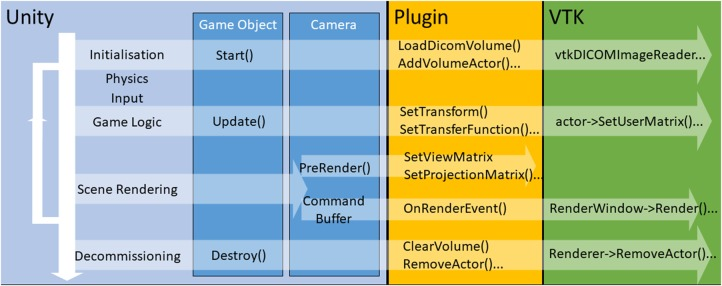
\includegraphics[width=\textwidth]{pictures/wheeler_architecture_zoomin.jpg}
    \caption{Wheeler et al.'s script handling of the VTK event loop.}
    \label{fig:wheeler-architecture-zoomin}
\end{figure}


\chapter{Design}
\label{ch:design}

This chapter introduces the architecture we developed based on the discussion of the requirements and challenges from Chapter~\ref{ch:rqrmsandclngs}. We discuss in detail the implementation of the core components that make the backend of our solution, as the most critical challenge we aim to tackle is to achieve the required performances to make our software usable. We will also discuss the frontend's design, in order to complete our discussion of the architecture, but its implementation and related challenges are out of the scope of this thesis.

%This chapter introduces the design choices implemented in our solution in order to overcome the challenges presented in Chapter~\ref{ch:unmaintainability}. We also discuss the implementation of the most critical aspects of this solution. We do not discuss the \acrshort{ui} implementation as it is out of the scope of this thesis. However, we will still discuss its design as it is part of the architecture we present and tackles some important points that are part of the requirements for the environment we are developing.

%This chapter presents the challenges encountered creating the system, what the most critical components are and the choices we made to overcome said issues. We first present the components that build up the system, what their responsibility are and the choices that lead us to this design. Then tackle each component one by one, focusing separately on each challenge. Afterwards we combine all the choices and present the final architecture of the system developed.

\section{Components}
\label{sec:components}

Based on our discussion of the challenges in Chapter~\ref{ch:rqrmsandclngs}, we opt for an architecture with components that each have a precise separate concern \cite{Hursch95separationof}. This stems from maintainability driven considerations arising from previous work's code, where components were highly coupled with both the visualization library and the engine \cite{dreuning_visual_2016, duking_potential_2018, kruis_creating_2017}. On the other hand, VtkToUnity already implements its code separating the Unity interface from the VTK and visualization logic within the plugin, moving most of its complexity in the C\# scripts.

The most basic design of our architecture requires two main endpoints, that are \acrshort{vtk} and Unity, a native layer of interfacing between the two and a managed Unity plugin to manage the invocation of native code from managed level and to implement the VR app's logic. The bare bones implementation was developed by Wheeler et al. \cite{wheeler_virtual_2018}, on which our solution is based. This gives us an infrastructural basement on which our further components are then built.

To achieve our goal of full integration of VTK, we cannot rely on hardcoded functions, which would impair the generality of the system, as well as its maintainability. As such, our solution comprises an introspecting component that enables the gathering of metadata on \acrshort{vtk} and thus limits the coupling of the solution to a particular version of \acrshort{vtk}.

On the other hand, the expression of such metadata also needs to be lowly coupled with the particular implementation of \acrshort{vtk}, and as such a component is introduced to enable the generation on-the-fly of UI that fits the I/O operations required to support the development environment. The design of the UI parts themselves is out of the scope of this thesis; we will only discuss its design, which enables the creation of the UIs.

Finally, this generality may come at the price of performance as introspection may be slow and interfacing may not be complete through it, as we discuss in Section~\ref{sec:design-introspection}, and the UI generation may be slow when working with big and complex pipeline filters. A first experiment in Section~\ref{sec:rqrmsandclngs-validation} shows that the performance on the creation of a somewhat complex pipeline using introspection, which yielded promising results. However, these performances may not be enough in all cases to support the use we envision for this software. As such, to enable users to enhance their experiences, both  tailored, more user-friendly UIs as well as focused and efficient adapters that create a direct link between the infrastructure and \acrshort{vtk} features are introduced in the architecture.

The final architecture is composed of a total of six components, as shown in Figure~\ref{fig:high-level-architecture}:

\begin{itemize}
    \item An \textbf{Infrastructure Layer} which acts as bridge between \acrshort{vtk} and Unity;
    \item A \textbf{\acrshort{vtk} Interfacing Layer}, comprised of an \textbf{Adapter Interface}, which uses custom made code by the user to interface with \acrshort{vtk}, and an \textbf{Introspection Interface}, which uses introspection over \acrshort{vtk} to access its features;
    \item A \textbf{Unity Managed plugin} which allows Unity to access the functionality exposed by the \textit{Infrastructure Layer};
    \item A \textbf{Unity UI Library}, comprised of a \textbf{UI Toolbox}, which is made of custom UIs created to tailor specific usages, and a \textbf{UI Composer}, which uses a minimal set of UI components to generate UIs on-the-fly.
\end{itemize}

\begin{figure}[t]
    \centering
    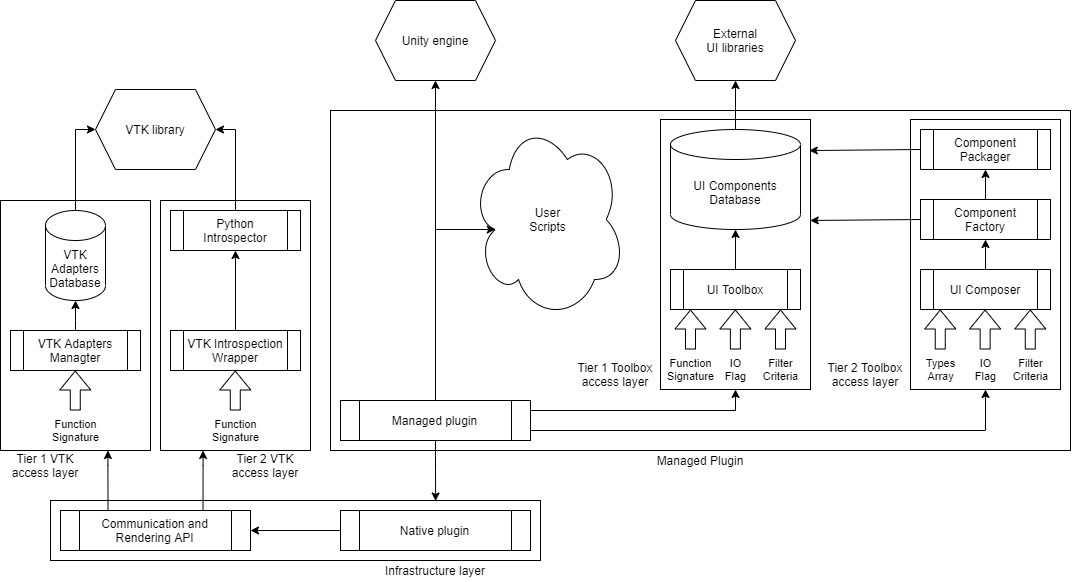
\includegraphics[width=\textwidth]{pictures/Architecture-v0.3.png}
    \caption{The architecture design of the plugin, showing inner working details of the various components.}
    \label{fig:high-level-architecture}
\end{figure}

\section{Infrastructure}
\label{sec:design-infrastructure}

The first component we tackle is the most simple yet the most crucial of this plugin. The infrastructure layer acts as a dispatcher for the requests coming from the managed plugin, routing them either to the rendering API or further down towards the VTK access components. As a reference, the component is highlighted in the architecture in Figure~\ref{fig:arch-infra}

\begin{figure}
    \centering
    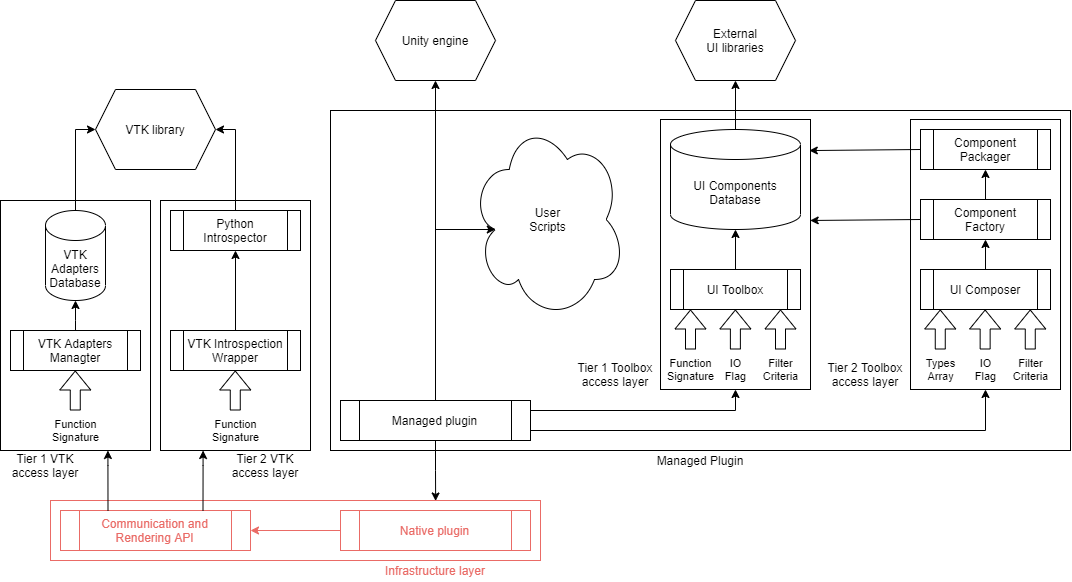
\includegraphics[width=\textwidth]{pictures/Architecture-v0.3-infra.png}
    \caption{Architecture with the infrastructure layer highlighted.}
    \label{fig:arch-infra}
\end{figure}

The infrastructure layer is the component responsible for allowing interaction between all other parts of the system. Its main job is to give a common entry-point to the \acrshort{vtk} interfaces and decide which to call, acting as a dispatcher. As this is the critical point of the system where communication flows, it is also the one that mostly affects parallelization and distribution capabilities. Thus, the calls should be as little blocking as possible, allowing flows to stop only at endpoints and not in the middleware.

Wheeler et al.'s VtkToUnity \cite{wheeler_virtual_2018} already partly implements this infrastructure layer and already exposes part of the \acrshort{vtk} interface as well. Unfortunately, their calls are highly blocking, as once the C++ native code executes, the Plugin calls each \verb|lock()| on the API and thus parallel calls are impossible. On the other hand, the plugin achieves decent performances that fall within the Unity guidelines for \acrshort{vr} \cite{unity_vr_2020}, while allowing for good maintainability and extension possibilities.

As such, we base the infrastructure layer on a refactoring of the VtkToUnity plugin which aims at the following results:

\begin{enumerate}
    \item Decoupling of the communication and dispatching from the interfacing responsibilities;
    \item Refactoring the interfacing code in adapters that constitute the foundation of the adapter-based interfacing;
    \item Move as much business logic of the infrastructure in non-blocking calls, preferably with no blocking at the infrastructure layer;
    \item Move blocking logic at interface level.
\end{enumerate}

%As we expect the interfacing to be slower, especially with the introspection component, the infrastructure layer will also have a cache system to store and retrieve the latest hits and directly call the precise function rather than going through with the introspecting dispatch system.

We use the same approach as in the VtkToUnity plugin to create the C++ native plugin and its interfacing with Unity. Our implementation is then reduced to the minimal API necessary to use the \acrshort{vtk} functionality expressed by the interface mechanisms described in Section~\ref{sec:design-interfaces}. Our objective is to make the calls as general as possible, giving the user the most liberty and access as possible. For the naming and implementation, we follow a similar design as the Python/C API \cite{python_c_api}. The interface is documented in Appendix~\ref{apx:api}.

In order to keep the readability and intuitiveness of the system decent, we apply this same approach to the API of all components. This is to limit the parsing operations, so that middleware has to apply as little transformation to the parameters as possible, as well as to make the maintainability of the system easier, as understanding data flows and meaning of values becomes easier with consistent naming and patterns.

\section{VTK Interfaces}
\label{sec:design-interfaces}

The core feature of our system is its ability to access \acrshort{vtk} and expose it fully to the \acrshort{vr} development environment. To achieve this, while keeping the system easily maintainable and performing, we use a two way access system. The first access route uses a lookup to check whether custom adapters exist that can satisfy the request from the caller, while the second uses introspection capabilities on the library to find the appropriate method, function or class that can satisfy the request.

We discuss both access tiers and how each of them is designed. Both these subsystems are intended to be separate services that the main architecture can either directly access when running in a stand-alone version on the users PC, or can be distributed on a network and be accessed through distribution engines such as DtCraft \cite{huang2017dtcraft} or Boost::MPI \cite{schaling2011boost}.

In order to limit the amount of routes in the infrastructure level and overheads, the interfaces follow a strict prioritization policy. The first tier is the Adaptrs registry, where a number of custom written adapters can be added and used by the plugin. If the infrastructure finds a suitable adapter, it will use it to answer the request. If no adapter is available, the query will be sent to the Introspection layer to be computed. However, if an adapter is found but it cannot satisfy the request, the system will not query the Introspection layer. Instead, it will return an error and it will be the user's responsibility to either query the Introspection layer directly or to expand the adapter. Other than the performance rationale behind this choice, the other main reason is that complexity in our system is kept at the peripheral components, with the clear intent of the dispatcher to be as simple and straight-forward as possible, limiting complexity in that central middleware.

\subsection{Introspection}
\label{sec:design-introspection}

The introspection layer is the low priority of the two VTK access tiers. It acts as the main route to connect to VTK and access its features and the most used component of the native part of our plugin for the average use-case of this system. It is comprised of two main parts, the Python \verb|Introspector| script, which uses the Dreuning implementation to access VTK introspectively, and the C++ wrapper that handles the memory used by the VTK objects and the Python Interpreter embedded in the system. As a reference, the component is highlighted in the architecture in Figure~\ref{fig:arch-intro}

\begin{figure}
    \centering
    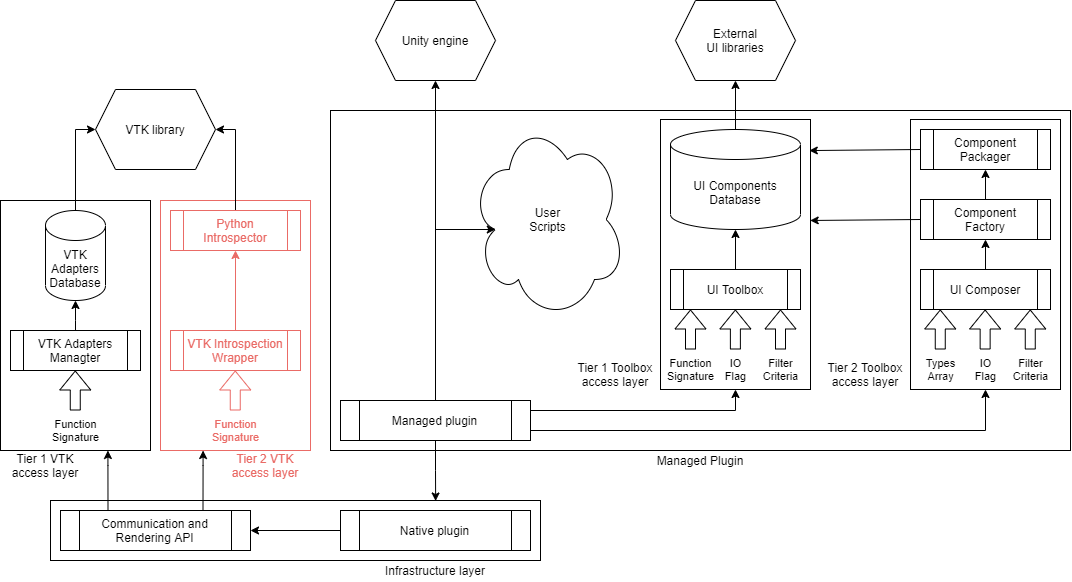
\includegraphics[width=\textwidth]{pictures/Architecture-v0.3-intro.png}
    \caption{Architecture with the introspection layer highlighted.}
    \label{fig:arch-intro}
\end{figure}

\subsubsection{Design}

As we discussed in Section~\ref{sec:rqrmsandclngs-challenges}, solutions already exist that implement introspective systems to access VTK in Python. In particular, we modify and extend the Python scripts from Dreuning's solution in order to make use of its \verb|ClassTree|. The issue we find with this implementation is that it is limited to \verb|vtkAlgorithm| classes, and as such leaves out a chunk of the features of the VTK. As extending these scripts is out of the scope of this thesis, we instead introduce a feature to overcome this limitation that would nevertheless be implemented, i.e. the ability to pipe the result of a VTK call to other calls. This does not allow the user to instantiate objects of classes that are not \verb|vtkAlgorithm|, however it allows already for a big part of the left out features to be accessed.

From Dreuning's solution we adapt the \verb|ClassTree| implementation in order to strip it of its UI related code, as well as the \verb|PipelineObject|, which we use as the introspective wrapper for the \acrshort{vtk} objects we instantiate to hold the getter and setter calls. A further script has been produced to facilitate the calls from C++, exposing the required features for: (a) creating a (wrapped) \acrshort{vtk} object and return the C++ object's address; (b) getting the description of a \acrshort{vtk} object, i.e. its attributes and their types, used by the Composer to generate UIs on-the-fly; (c) get the value of a \acrshort{vtk} object's attribute; (d) set the value of a \acrshort{vtk} object's attribute; and (e) delete the wrapper's information once the \acrshort{vtk} object gets deleted in the environment. 

In order to access the Python scripts from the C++ native plugin, we embed the Python 3.7 interpreter in the C++ implementation. This is achieved by initializing the interpreter as part of the process, using a subset of the software's memory to run Python. This, combined with the ability to wrap the C++ VTK objects using the \verb|vtkPythonUtils| class into Python and then access them back again, allows us not to worry about synchronizing memory and processes, boosting both memory and time performances.

The implementation instantiates a \verb|Introspector| class from Python, using it as access-point for the introspective methods. Using the \verb|PyObject_CallMethod| we are able to use the methods of the \verb|Introspector|, starting with \verb|createVtkObject| which instantiates a wrapped VTK object, using the class name, that carries the information of the getter and setter methods of the \verb|vtkAlgorithm| class. These wrapped objects, that we will now call \textit{nodes}, are registered in a structure that maps the pointer of the C++ object to its wrapped Python counterpart, for fast lookup access \cite{stdunord16}. The C++ interface exposes calls that allow, having the node available, to call getters, setters, to execute the VTK update of the object, retrieve the output port, delete the object, execute a generic or piped call. This last one means that you can execute, for example, \verb|object.GetOutput().GetCenter()| with a single access to the \verb|Introspector| and use non introspectable objects as intermediate values, expanding the possible calls that the plugin can execute.

To avoid ambiguity when calling these methods, and to avoid passing excessive data through the Unity native interface, the methods that retrieve values from the \verb|Introspector| use a postfix notation to determine whether the call is to return a native value that can easily be parsed to and from a string representation (\verb|_AsString|), an id of a VTK object (\verb|_AsVtkObject|), or either if the result is to be discarded or the method being called has \verb|void| return type (\verb|_AsVoid|).

When calling any method that uses parameters of generic types, we use a similar convention as the Python/C API so to make the maitainability of the code easier, as these are strictly intertwined and usually used alongside. As such, calls are structured as follows: the first parameter is the pointer to the object on which the method is to be called, the second parameter is the name of the method to be called, or a specifier that acts as a dispatching value (i.e. dispatching either to \verb|SetInputConnection| or \verb|SetSourceConnection|), third is the string format of the following parameters (e.g. a method that has three doubles as parameters would have as format \verb|"fff"|), and finally a vector containing the parameters. Special treatment is reserved for the \verb|"O"| object parameters that are first past as string representation of integer values, then parser to integers by the infrastructure layer, which represents the id of the VTK object in the registry, and finally two vectors are sent to the introspection layer, one with the \verb|vtkObjectBase *| objects and the other with the rest of the parameters.

A complete description of the formatting values see Table~\ref{tab:format-values}, while the interface of the introspection layer is documented in Appendix~\ref{apx:api}

\begin{table}[t]
    \centering
    \begin{tabulary}{.9\textwidth}{LL}
    \multicolumn{1}{c}{\textbf{Symbol}} & \multicolumn{1}{c}{\textbf{Meaning}} \\ \hline
    O & A VTK object. The value from the Managed plugin is the ID of the object in the infrstructure layer's registry. The Introspection layer receives the pointer to the VTK object. \\
    d                                   & A C integer or long value.           \\
    f                                   & A C float or double value.           \\
    s                                   & A C char or LPCSTR value.            \\
    b                                   & A C++ bool value.                    \\
    \%\# & is any of the previous symbols, \# is the number of values. It represents a tuple of values, e.g.: f3 corresponds to (fff) in the Python/C API.
    \end{tabulary}
    \caption{Format symbols used in the calls to the plugin.}
    \label{tab:format-values}
\end{table}

\subsubsection{Benefits and Limitations}

The obvious benefit of this implementation is that it allows us to broadly achieve VTK-completeness in our system. The Python component gives the plugin access to the \verb|vtkAlgorithm| classes, and through piped calls to VTK it is possible to implement virtually any visualization a native application could make. The Introspector can instantiate all the necessary VTK objects using the \verb|genericCall| at Python level and as such it could potentially make the system strictly VTK complete. However, this would come at a great cost in terms of computation time, as all the information available for the \verb|vtkAlgorithm| classes is not generated.

A more subtle benefit of the usage of Python is that it is an interpreted language, and the interpreter being embedded in the C++ code makes it easier to maintain and expand the Introspector capabilities. Changes to such parts of the introspection layer would not require the plugin to be re-built everytime, whereas any change to the C++ code requires the plugin to be built and deployed in the Unity environment again. Furthermore, Python being a high level language, the actual implementation becomes more readable and understandable, making the component easier to work on.

As already introduced in Section~\ref{sec:design-infrastructure} on the infrastructure layer, we use a common convention on functions' and parameters' names and meaning, very similar to the Python/C API. Keeping this standard is not only beneficial to the maintainability of the system, as the code is easier to read, but also to its performances as the passage from our C++ to the Python/C API calls and viceversa is straight-forward, requiring limited parsing.

The API proposed does not limit the users ability to use VTK. Indeed, the calls that are exposed make no assumption on what the objects are used for and how, and they create as little barriers as possible. The main issue is that the calls support only a limited amount of types as parameters, compared to the Python/C API. On the other hand, these are representative of most of the types used within VTK classes and as such we believe this to be a minor limitation and that it does not impair our solution.

Lastly, thanks to the fact that most of the implementation of the C++ introspection layer uses little classes from VTK and mostly classes that tend to be not modified a lot by the VTK developers, like the \verb|vtkObjectBase| class, which is the root of all classes in the library. As such, updating the component to newer versions of VTK requires only the recompilation of the plugin and having the correct version of the Python wrapper installed on the machine.

The main limitation of this implementation is that it is not strictly VTK complete. Any class that is not inheriting from \verb|vtkAlgorithm| is not introspected on. These classes could be made available through generic calls through Python, but this would potentially introduce overheads at runtime that are not acceptable in such a performance critical system. As such, we accept this limitation of the system as it makes for a good compromise between our requirements of VTK completeness and performance. And thanks to the fact this is all achieved through Python, the system could potentially be made strictly VTK complete without touching the C++ code and as such left for future work.

\subsection{Adapters}
\label{sec:design-adapters}

Next to the introspection layer, the adapter layer is comprised of a collection of adapters added by the user. These are a way of allowing users to expand the plugin, taking advantage of the pure C++ performance edge over the C++ and Python introspection layer. Furthermore, it allows the users to introcude "templates" in the plugin, i.e. creating adapters that reduce repetitive and verbose calls to a single call to the C++ plugin. As a reference, the component is highlighted in the architecture in Figure~\ref{fig:arch-adapt}

\begin{figure}
    \centering
    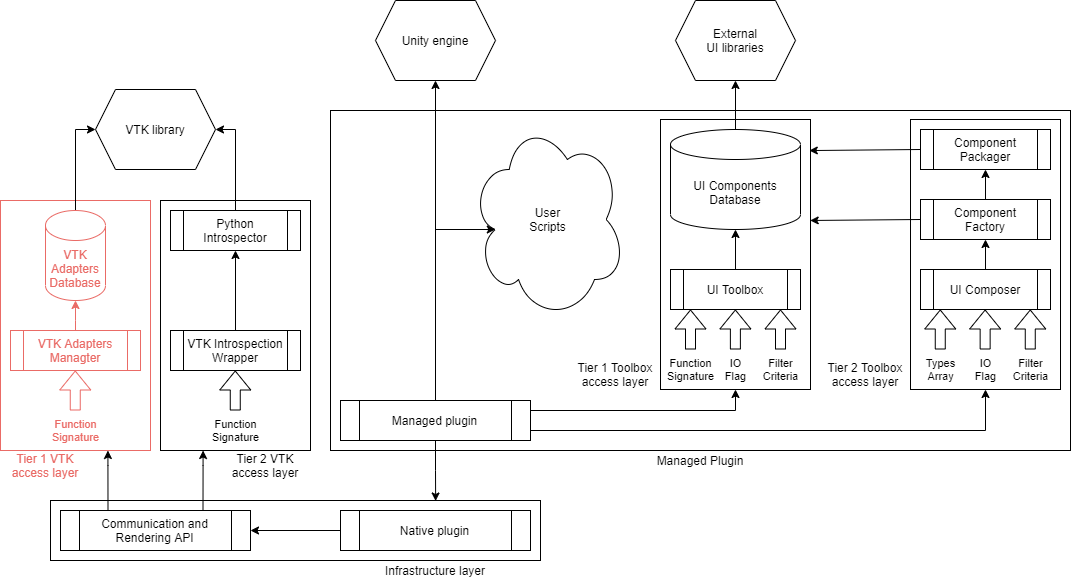
\includegraphics[width=\textwidth]{pictures/Architecture-v0.3-adapt.png}
    \caption{Architecture with the adapter layer highlighted.}
    \label{fig:arch-adapt}
\end{figure}

\subsubsection{Design}

The adapter layer is one of the two main ways in which expert users can tailor their experience with the system. These are pieces of C++ code that can be introduced in the native plugin's adapters folder and be called from the Unity environment. Particular use cases for adapters are:

\begin{enumerate}
    \item The creation of custom loggers for diagnostics and flow analysis;
    \item Implementation of \textit{templates} at native level that enable faster instantiation and define their own parameters and routines;
    \item Implementation of custom algorithms that compound \acrshort{vtk} features.
\end{enumerate}

The adapters are Singleton instances that define first and foremost a unique string identifying which component they are adapting. Such ID represents the name of the object the code adapts. For instance, an adapter for the  source class \verb|vtkConeSource| should be identified by the class' name. Furthermore, each adapter has to implement access methods for getting descriptions of what attributes the class has, getting the values of each of those attributes and setting such values as well. 

Optionally, the adapter can implement rendering information in case the adapter is not for a specific \acrshort{vtk} class but for a template or custom algorithm, in which case information is needed on how to render and update the objects generated by the adapter.

In order to implement the defined adapters, we first define a basic adapter class which is used for only use case number 1, i.e. the adapting of \acrshort{vtk} defined objects. This class does not define rendering and update information, as these are already defined by \acrshort{vtk}. We implement \verb|vtkAdapter| as shown in listing~\ref{lst:vtkadapter}

\begin{figure}[ht!]
    \centering
    \begin{cpp}[label=lst:vtkadapter,caption={vtkAdapter class}]
class vtkAdapter
{
public:
    template <typename T> using getter = std::stringstream(T::*)(vtkObjectBase *);
    template <typename T> using setter = void (T::*)(vtkObjectBase *, LPCSTR);

    virtual ~vtkAdapter() { }

    inline LPCSTR GetAdaptingObject() 
    {
        return m_vtkObjectName;
    }

    virtual void SetAttribute(
        vtkObjectBase *object,
        LPCSTR propertyName,
        LPCSTR newValue) = 0;

    virtual LPCSTR GetAttribute(
        vtkObjectBase *object,
        LPCSTR propertyName) = 0;

    virtual LPCSTR GetDescriptor() const = 0;

    virtual vtkObjectBase *NewInstance() = 0;

    virtual LPCSTR CallMethod_AsString(
        vtkObjectBase *object,
        LPCSTR method,
        LPCSTR format,
        const char *const *argv) const = 0;

    virtual vtkObjectBase *CallMethod_AsVtkObject(
        vtkObjectBase *object,
        LPCSTR method,
        LPCSTR format,
        const char *const *argv) const = 0;

    virtual void CallMethod_AsVoid(
        vtkObjectBase *object,
        LPCSTR method,
        LPCSTR format,
        const char *const *argv) = 0;

protected:
    // The name of the VTK object (as written in the wiki) for which
    // the class acts as an adapter
    LPCSTR m_vtkObjectName;

    vtkAdapter(
        LPCSTR vtkObjectName) 
    { 
        m_vtkObjectName = vtkObjectName;
    };
};
    \end{cpp}
\end{figure}

The class has a unique identifier in the form of a \verb|LPCSTR| (Long Pointer to Const STRing) which is to be set when instantiating the adapter. The class also carries with it a descriptor of the \acrshort{vtk} class that specifies what attributes the class has and what is their type. This descriptor is used by the Unity Managed plugin as we discuss in Section~\ref{sec:design-uicomposer}.

Alongside these functions, there are two templates that define the types of \verb|getter| and \verb|setter| methods used by adapters. These functions take as input a pointer to the actor that renders the \acrshort{vtk} object and the first returns a string representation of the value of the attribute while the second takes a further argument that is the new value to which attribute is to be set.

The generic calls for getting and setting attributes are respectively \verb|GetAttribute| and \verb|SetAttribute|. These functions act as dispatchers for the particular operations, that can either be directly implemented into the function but, as good practice, we later show an example of how we recommend these adapters should be implemented.

The actual attribute to change is encoded in a \verb|LPCSTR| that contains the name of the attribute exactly as written in the C++ code. A difference from the \verb|GetAttribute| generic call and the particular \verb|getter| template is that the return value is not returned but a specific parameter acts as return buffer, as this value is not to be used inside the C++ native code but to be sent through to the C\# interface in Unity.

Finally, the \verb|CallMethod| family of methods allows the user to implement generic methods that can be called from the Unity environment. In particular, these methods are meant to be used to accomodate the needs of use cases number 2 and 3. These use a similar signature to the \verb|VtkResource_CallMethod| methods from the plugin's API, so that the parameters can be directly passed down without the need of unnecessary parsing at the infrastructure level. The responsibility for correct parsing is left to the user to implement, so that they can also have a higher degree of freedom of what they can actually code.

Alongside the adapters, the \verb|vtkAdapterUtility| provides the access point for the register of the adapters. This allows to couple adapters to a single point of entry and masks the adapters to the infrastructure layer, making it easy to execute on a separate service. The implementation of this class is generated by a Python script at build time, available in Appendix~\ref{apx:generate-register}. The interface of the utility is shown in Listing~\ref{lst:vtkadapterutility}.

\begin{figure}[ht!]
    \centering
    \begin{cpp}[label=lst:vtkadapterutility,caption={vtkAdapterUtility interface}]
class vtkAdapterUtility
{
public:
	static vtkAdapter *GetAdapter(LPCSTR vtkAdaptedObject);

private:
	static const std::unordered_map<LPCSTR, vtkAdapter *> s_adapters;
};
    \end{cpp}
\end{figure}

As visible, the adapter only exposes the function \verb|GetAdapter| that returns the implementation of the adapter for the unique ID requested if such object exists, \verb|NULL| otherwise. The adapters are stored in an unordered map, as it has faster access times than the ordered counterparts \cite{stdunord16, stdmapcp55} on the average case. This depends on the hashing function, but as we use default types for keys and we do not replicate them, the average case is almost certainly guaranteed. The map is populated on instantiation and the entries are generated as Singletons, as shown in Listing~\ref{lst:adaptersmap}.

\begin{figure}[ht!]
    \centering
    \begin{cpp}[label=lst:adaptersmap,caption={Example of adapters register instantiation.}]
const std::unordered_map<LPCSTR, vtkAdapter*> vtkAdapterUtility::s_adapters =
{
	{ Singleton<vtkConeSourceAdapter>::Instance()->GetAdaptingObject(), Singleton<vtkConeSourceAdapter>::Instance() },
	// More adapters...
};
    \end{cpp}
\end{figure}

\subsubsection{Benefits and Limitations}

These adapters have the objective of allowing the user to customize their system and tailor it to their needs. The user can define different ways in which the native plugin interacts with \acrshort{vtk}. The ability to customize the software to this extents enables users to create code that can be re-used and distributed. Within a community of users, this allows them to exchange knowledge and tools that could not be achieved without this feature.

The main driver behind adapters is to make the solution maintainable as well as generic. We do not foresee all potential uses of the adapters, as it is not our objective. Their implementation is kept to the bare minimum and some use cases are presented which are, to us, the most obvious. We set out to not limit the potential for these components, and require the implementation of what is needed to make it work. This caters to our requirement of a usable system, as it makes it easier to tailor to specific needs of users.

The level of generality of this component however is also one of its main limitations. As we cannot foresee all the possible use-cases, and to avoid limiting users' options, we do not enforce many restrictions on what adapters can and cannot do. Furthermore, we can do little to enforce standards and recommended ways of using adapters, for the same reasons as before. As such, where users have great potential for new features, thay also have little support from the system to maintain and debug them.

Another limitation, at least compared to the introspection layer, is that this tier has no guarantee to compile with different versions of VTK, as the features used are not guaranteed to be present or be the same across versions. Although VTK developers have as one of their requirements the new versions of the library to be backwards compatible as already discussed in Chapter~\ref{ch:rqrmsandclngs}, this does not mean that they are forwards compatible, and adapters developed with newer versions of VTK are not guaranteed to work with older ones, and we do not set a way to solve this issue. This is because adapters are tools for the users and they should be responsible for paying attention to these kind of details.

The other great advantage of adapters over introspection is that it can make use of the performances of pure C++ code. As we discussed in Chapter~\ref{ch:rqrmsandclngs}, pure C++ code runnig VTK algorithms achieves far greater performances on the execution of pipelines than our approach using Python. As such, adapters enable the users to take advantage of such performances, removing the barrier of also having to code their Unity plugin along.

\section{Managed Plugin}
\label{sec:design-managed-plugin}

The integration of VTK with Unity makes use of both a native plugin, which we already discussed, and a managed plugin, which is the focus of this section. In particular, this part of the system is responsibile for making the native plugin API more user-friendly, and connecting the rendering cycles of the two rendering contexts. The setup is almost identical to the VtkToUnity plugin, with a different API for VTK.

The basic API of the managed plugin is identical to the native plugin API, with the exception of the usage of the \verb|Marshal|, a .NET library used to work with unmanaged memory areas. In Unity, this library is used in particular to handle passing paramters back and forth between the managed and native parts of the environment, like defining how strings have to be handled passing down to C++. In our implementation we use this exclusively to specify strings to be handled as long pointer strings, as we represent them as \verb|LPCSTR| (Long-Pointer Constant STRing) in our C++ code.

As a further design discussion, we present now the Toolbox and Composer components that are part of the managed plugin. As the UI is out of the scope of this thesis, we will not discuss particular implementations of these components, as they will be presented in a separate thesis. Designing these components, we mirror our approach to accessing VTK, as our drivers remain the same. In particular, the Toolbox is the component that mirrors the Adapters registry, while the Composer mirrors the Introspector.

For the API of the managed plugin, see Appendix~\ref{apx:api}. The minimal API is identical to the native plugin API, with the types being those of C\#, while the support and quality of life methods introduced in C\# to avoid verbose code is separately documented.

\subsection{UI Toolbox}
\label{sec:design-toolbox}

The UI Toolbox is the main access to UI components of the managed plugin. It acts as a database of factories that generate specific UIs when called upon. As a reference, the component is highlighted in the architecture in Figure~\ref{fig:arch-toolbox}

\begin{figure}
    \centering
    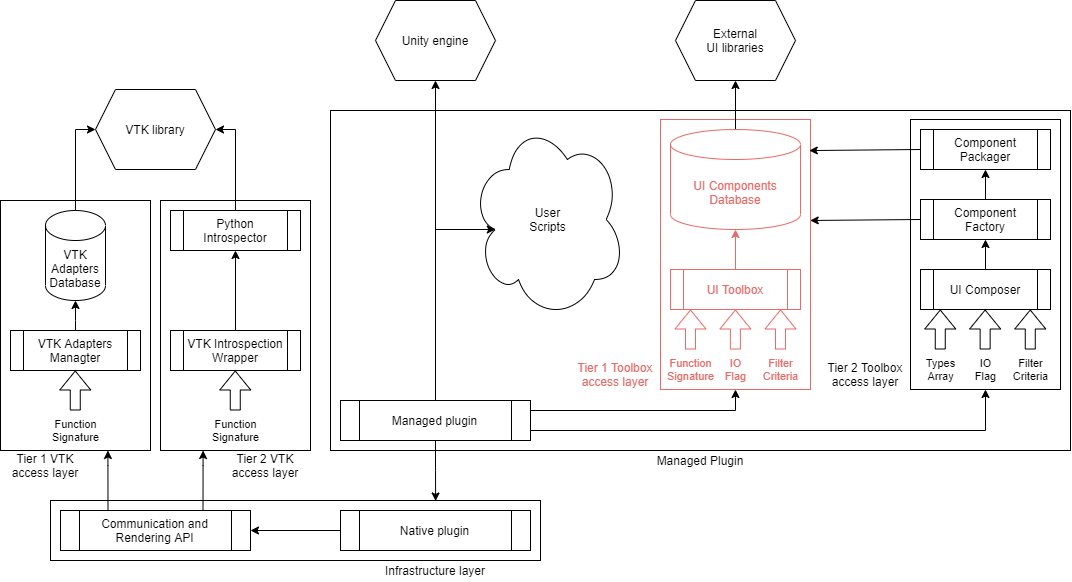
\includegraphics[width=\textwidth]{pictures/Architecture-v0.3-toolbox.png}
    \caption{Architecture with the UI Toolbox highlighted.}
    \label{fig:arch-toolbox}
\end{figure}

As UIs are in general more complex than accessing introspectively a library, as they are made of more components and constrained by interaction and usage limits that depend on the device being used, the environment, the input devices and so on, the ability to introduce custom-tailored UI components is necessary. Thus, we propose the usage of a registry of UI prefabs developed in Unity as first-tier access to the UI of the environment.

A registry mapping from the classname to the prefab factory \verb|IComponentFactory| acts as the access-point for the UI instantiation. When a part of the pipeline is created, the \verb|FactoryManager| first checks the registry to check whether a factory for the entire UI exists. If this exists, the factory is called and a \verb|Create| function generates the UI based on the prefab. The UI is then linked to the particular part of the pipeline by the manager in order to keep track of the changes and to avoid the changes being either lost or set to the wrong VTK object. This is also to have the UI ready but not shown, and only made visible through \verb|Show| when necessary and hidden through \verb|Hide| when changing focus.

\subsection{UI Composer}
\label{sec:design-uicomposer}

Finally, the UI Composer is the last part of the plugin we will discuss. This is a factory of factories, generating UI components that are a collection of minimal input UIs that are the base of the UI Toolbox. As a reference, the component is highlighted in the architecture in Figure~\ref{fig:arch-comp}

\begin{figure}
    \centering
    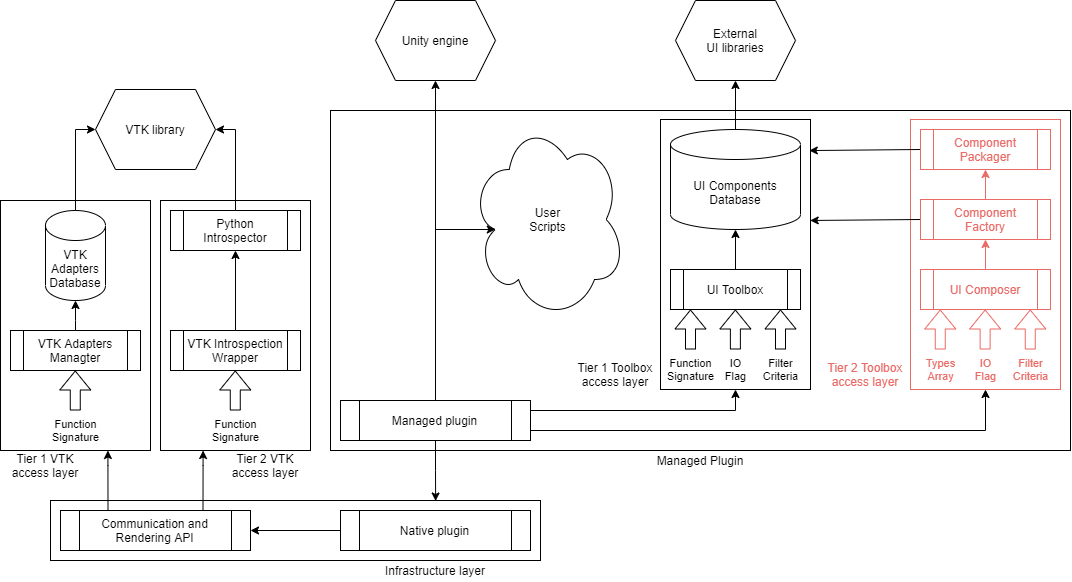
\includegraphics[width=\textwidth]{pictures/Architecture-v0.3-comp.png}
    \caption{Architecture with the UI Composer highlighted.}
    \label{fig:arch-comp}
\end{figure}

If the Toolbox fails, a generic system to generate UIs gets called. This requires more resources and time to execute, as it takes the descriptor of the VTK object, which maps the names of the attributes to their types, and then creates a minimal UI with this information. The Composer uses a registry of minimal components that are part of the environment that implement interfaces to edit native simple values, e.g. integers, decimals, booleans, strings and so on. These components are also registered with the Toolbox, for faster access.

The components generated this way are then used to instantiate a \verb|ComposedUI| object, that contains the information of the different parts that make the UI and then add this to the Composer's registry, acting as a \verb|IComponentFactory| for later calls of the \verb|FactoryManager| on the same classname to avoid generating the same factory twice.

In order to accelerate and expand the Composer's ability, the mappings are not hardcoded; the Composer still uses the Toolbox as a lookup for the basic parts used to generate the UI, and thus custom-tailored basic UIs can be added to the Toolbox to override the natively implemented ones. In this way, the component for a given string in the \verb|FactoryManager|'s registry is always the last one registered, making the native ones the lowest priority ones.

The \verb|FactoryManager| is designed in order to accomodate our maintainability driver, and as such this modular registry comes in handy to set some conventions in the development of UIs using this system that make them re-usable. In particular, UI components should be registered either if they allow the manipulation and/or visualization of a single parameter or when they combine other UI components. The first ones constitute the minimal set of the UI components, which respond to a particular input/output, like \verb|float|, \verb|int|, or \verb|string|, while the others respond to complex interactions like showing the UI for a \verb|vtkConeSource| object, or visualizing a \verb|stringList|. For the naming of the components we encourage camel case with the first letter lowercase as by VTK's convention. 

This conventions also make for the best operability of the Composer that will be able to generate more complex UIs, using composed UIs instead of simple input methods. To allow for further customization, we propose that the names can be postponed with filters that specify how the input is inserted, i.e. a float can be inputted through \verb|slider| or \verb|textField| for example. However, this is to make the modularity more useful to the user, rather than to the composer, as we do not design how these filters could be used by it.

\chapter{Results}

\label{ch:results}
In this chapter, we present the results of our experiment(s). 


\chapter{Discussion}
\label{ch:discussion}
In this chapter, we discuss the results of our experiment(s) on ...

\begin{finding}
	Highlight like this an important finding of your analysis of the results.
	\label{find:important1}
\end{finding}

Refer to Finding~\ref{find:important1}.

\section{Threats to validity}
What could affect the validity of your research? Think of pitfalls of your research method, experimental setup, interpreting the results.




\chapter{Related work}
\label{ch:related_work}
We divide the related work into the following categories:  ...


\chapter{Conclusion}
\label{ch:conclusion}



\section{Future work}
\label{sec:future_work}

\chapter*{Acknowledgements}
If so inclined, thank people.

\printbibliography[heading=bibintoc]
\printglossaries%

\begin{appendices}

\chapter{Example VTK pipeline}
\label{apx:quadric-vtk}
	
\begin{cpp}[label=lst:quadricvtk,caption={Example of Quadric Contour in VTK.},aboveskip=20pt]
#include <vtkQuadric.h>
#include <vtkSampleFunction.h>
#include <vtkContourFilter.h>
#include <vtkOutlineFilter.h>
#include <vtkPolyDataMapper.h>
#include <vtkActor.h>
#include <vtkProperty.h>
#include <vtkRenderWindow.h>
#include <vtkRenderer.h>
#include <vtkRenderWindowInteractor.h>
#include <vtkImageData.h>
#include <vtkNew.h>
#include <vtkPolyData.h>

int main(int arc, char* argv)
{
	vtkNew<vtkQuadric> quadric;
	quadric->SetCoefficients(.5,1,.2,0,.1,0,0,.2,0,0);

	vtkNew<vtkSampleFunction> sample;
	sample->SetSampleDimensions(200,200,200);
	sample->SetImplicitFunction(quadric);

	vtkNew<vtkContourFilter> contours;
	contours->SetInputConnection(sample->GetOutputPort());
	contours->GenerateValues(5,0.0,1.2);

	vtkNew<vtkPolyDataMapper> contMapper;
	contMapper->SetInputConnection(contours->GetOutputPort());
	contMapper->SetScalarRange(0.0,1.2);

	vtkNew<vtkActor> contActor;
	contActor->SetMapper(contMapper);

	vtkNew<vtkOutlineFilter> outline;
	outline->SetInputConnection(sample->GetOutputPort());

	vtkNew<vtkPolyDataMapper> outlineMapper;
	outlineMapper->SetInputConnection(outline->GetOutputPort());

	vtkNew<vtkActor> outlineActor;
	outlineActor->SetMapper(outlineMapper);
	outlineActor->GetProperty()->SetColor(0,0,0);

	vtkNew<vtkRenderer> ren;
	vtkNew<vtkRenderWindow> renWin;
	renWin->AddRenderer(ren);

	vtkNew<vtkRenderWindowInteractor> iren;
	iren->SetRenderWindow(renWin);

	ren->AddActor(contActor);
	ren->AddActor(outlineActor);
	ren->SetBackground(1,1,1);

	renWin->Render();
	iren->Start();

	return EXIT_SUCCESS;
}
\end{cpp}
	
\chapter{VtkAdapterUtility code generator}
\label{apx:generate-register}
	
In order to generate at before build a register of all the adapters added to the plugin, a Python script has been created to automate this process. This will generate the necessary support class used within the plugin, i.e. \verb|VtkAdapterUtility|. This class is comprised of a fixed header file and an source file that changes depending on the installed adapters. The Listing~\ref{lst:generateheader} shows the code of such script. An example of generated source file is shown in Listing~\ref{lst:vtkadapterutilityex}

\begin{python}[label=lst:generateheader,caption={generate-header.py script},aboveskip=20pt]
import os

adapter_utility_h_name = "vtkAdapterUtility.h"
adapter_utility_cpp_name = "vtkAdapterUtility.cpp"
adapter_utility_class_name = "VtkAdapterUtility"
adapter_utility_getter_name = "GetAdapter"
adapter_utility_register_name = "s_adapters"
adapter_utility_register_type = "const std::unordered_map<LPCSTR, VtkAdapter*>"

adapter_utility_h = open(adapter_utility_h_name, "w")
adapter_utility_cpp = open(adapter_utility_cpp_name, "w")



### GENERATING HEADER FILE

adapter_utility_h.write("#pragma once\n")
adapter_utility_h.write("\n")
adapter_utility_h.write("/* This file has been automatically generated through the Python header generation utility\n")
adapter_utility_h.write(" * \n")
adapter_utility_h.write(" * This file contains the necessary information to allow the VtkToUnity plugin to know\n")
adapter_utility_h.write(" * that the adapters exist and it can call them. As such, this should be generated every\n")
adapter_utility_h.write(" * time the plugin is built to avoid losing any adapters in the compilation.\n")
adapter_utility_h.write(" */\n")
adapter_utility_h.write("\n")
adapter_utility_h.write("\n")

adapter_utility_h.write("// Utility includes\n")
adapter_utility_h.write("#include <unordered_map>\n")
adapter_utility_h.write("\n")
adapter_utility_h.write("#define NOMINMAX\n")
adapter_utility_h.write("#include <windows.h>\n")
adapter_utility_h.write("\n")
adapter_utility_h.write("#include \"../Singleton.h\"\n")
adapter_utility_h.write("#include \"../vtkAdapter.h\"\n")
adapter_utility_h.write("\n")


adapter_utility_h.write("\n")
adapter_utility_h.write("\n")
adapter_utility_h.write("// This class is used to register the adapters\n")
adapter_utility_h.write(f"class {adapter_utility_class_name}\n")
adapter_utility_h.write("{\n")

# Generating the class for the utility operations

adapter_utility_h.write("public:\n")

# begin public area

adapter_utility_h.write(f"\tstatic VtkAdapter* {adapter_utility_getter_name}(\n")
adapter_utility_h.write("\t\tLPCSTR vtkAdaptedObject);\n")
adapter_utility_h.write("\n")

# end public area

adapter_utility_h.write("private:\n")

# begin private area

adapter_utility_h.write("\t// Map with all the adapters registered in this folder\n")
adapter_utility_h.write(f"\tstatic {adapter_utility_register_type} {adapter_utility_register_name};\n")

# end private area

adapter_utility_h.write("};\n")



### GENERATING SOURCE FILE

adapter_utility_cpp.write("/* This file has been automatically generated through the Python header generation utility\n")
adapter_utility_cpp.write(" * \n")
adapter_utility_cpp.write(" * This file contains the necessary information to allow the VtkToUnity plugin to know\n")
adapter_utility_cpp.write(" * that the adapters exist and it can call them. As such, this should be generated every\n")
adapter_utility_cpp.write(" * time the plugin is built to avoid losing any adapters in the compilation.\n")
adapter_utility_cpp.write(" */\n")
adapter_utility_cpp.write("\n")
adapter_utility_cpp.write("\n")
adapter_utility_cpp.write(f"#include \"{adapter_utility_h_name}\"\n")
adapter_utility_cpp.write("\n")
adapter_utility_cpp.write("// Adapters' header files found in the folder (.h and .hpp)\n")

# Generating the includes of the adapters' header files

classes = []

for f in os.listdir("."):
    if f != adapter_utility_h_name and ( f.endswith(".h") or f.endswith(".hpp") ):
        adapter_utility_cpp.write(f"#include \"{f}\"\n")
        class_name = os.path.splitext(f)[0]
        classes.append(class_name[:1].upper() + class_name[1:])

adapter_utility_cpp.write("\n")
adapter_utility_cpp.write("\n")

# Creating the adapters' mapping

adapter_utility_cpp.write(f"{adapter_utility_register_type} {adapter_utility_class_name}::{adapter_utility_register_name} =");
adapter_utility_cpp.write("{\n")

# begin s_adapters init

for clss in classes:    
    adapter_utility_cpp.write(f"\t{{ Singleton<{clss}>::Instance()->GetAdaptingObject(), Singleton<{clss}>::Instance() }},\n")

# end s_adapters init

adapter_utility_cpp.write("};\n")

adapter_utility_cpp.write("\n")
adapter_utility_cpp.write("\n")

adapter_utility_cpp.write(f"VtkAdapter* {adapter_utility_class_name}::{adapter_utility_getter_name}(\n")
adapter_utility_cpp.write("\tLPCSTR vtkAdaptedObject)\n")
adapter_utility_cpp.write("{\n")

# begin GetAdapter

adapter_utility_cpp.write("\tauto itAdapter = s_adapters.find(vtkAdaptedObject);\n")
adapter_utility_cpp.write("\tif (itAdapter != s_adapters.end())\n")
adapter_utility_cpp.write("\t{\n")
adapter_utility_cpp.write("\t\treturn itAdapter->second;\n")
adapter_utility_cpp.write("\t}\n")
adapter_utility_cpp.write("\telse\n")
adapter_utility_cpp.write("\t{\n")
adapter_utility_cpp.write("\t\treturn NULL;\n")
adapter_utility_cpp.write("\t}\n")

# end GetAdapter

adapter_utility_cpp.write("}\n")
\end{python}
    
\begin{cpp}[label=lst:vtkadapterutilityex,caption={Example VtkAdapterUtility.cpp},aboveskip=20pt]
/* This file has been automatically generated through the Python header generation utility
 * 
 * This file contains the necessary information to allow the VtkToUnity plugin to know
 * that the adapters exist and it can call them. As such, this should be generated every
 * time the plugin is built to avoid losing any adapters in the compilation.
 */


#include "vtkAdapterUtility.h"

// Adapters' header files found in the folder (.h and .hpp)
#include "vtkConeSourceAdapter.h"


const std::unordered_map<LPCSTR, VtkAdapter*> VtkAdapterUtility::s_adapters ={
	{ Singleton<VtkConeSourceAdapter>::Instance()->GetAdaptingObject(), Singleton<VtkConeSourceAdapter>::Instance() },
};


VtkAdapter* VtkAdapterUtility::GetAdapter(
	LPCSTR vtkAdaptedObject)
{
	auto itAdapter = s_adapters.find(vtkAdaptedObject);
	if (itAdapter != s_adapters.end())
	{
		return itAdapter->second;
	}
	else
	{
		return NULL;
	}
}
\end{cpp}
    
\end{appendices}

%comment out in the final version
%\listoftodos[Notes]

\end{document}
